\documentclass[english]{tnreport}
%\documentclass[stage1a]{tnreport} % If you are in 1nd year
%\documentclass[stage2a]{tnreport} % If you are in 2nd year
%\documentclass[confidential]{tnreport} % If you are writing confidential report
%\documentclass[english]{tnreport} % If you are writing your report in english
%\documentclass[contratpro]{tnreport} % If you are in contrat pro

\def\reportTitle{Winter is Coming} % Titre du mémoire
\def\reportLongTitle{Winter is Coming --- You know nothing Jon Snow} % Titre plus long du mémoire

\def\reportAuthor{Jon Snow}
\def\reportAuthorEmail{\email{jon@castleblack.com}} % Courriel de l'élève

% Signatures
\addSignaturesLine{{
  {figures/anonymous_company-logo}{Jon SNOW}{Élève-ingénieur},
  {figures/anonymous_company-logo}{Eddard STARK}{Gouverneur du Nord}
}}

% Si d'autres personnes doivent/veulent signer le rapport (encadrant académique...), ajouter des lignes :
%\addSignaturesLine{{
%  {figures/anonymous_company-logo}{Tyrion LANNISTER}{Main du Roi},
%  {figures/anonymous_company-logo}{Tywin LANNISTER}{Gouverneur de l'Ouest},
%  {figures/anonymous_company-logo}{Jaime LANNISTER}{Lord Commandant,\\Garde Royale}
%}}

% This is an example, for a report with several students as authors
%\def\reportAuthor{Jon Snow\\ Samwell Tarly}
%\def\reportAuthorEmail{\email{jon@castleblack.com}\\ \email{tarly@casteblack.com}} % Courriel de l'élève

\def\reportAuthorAddress{numéro, rue} % Adresse de l'élève
\def\reportAuthorCity{code postal, VILLE} % Adresse (cont.) de l'élève
\def\reportAuthorPhone{téléphone} % Téléphone de l'élève

%\def\reportIndustrialSupervisor{Eddard Stark} % Prénom Nom de l'encadrant industriel
\def\reportSupervisor{Eddard Stark} % Prénom Nom de l'encadrant industriel (en entreprise ou laboratoire)
\def\reportAcademicSupervisor{Tyrion Lannister} % Prénom Nom de l'encadrant académique

% For PIDR ?
%\def\reportSupervisor{Eddard Stark} % Prénom Nom de l'encadrant industriel
%\def\reportProjectCustomer{Projet réalisé pour l'équipe Night's Watch du laboratoire HBO}

\def\reportCompany{Home Box Office} % Nom de l'entreprise d'accueil
\def\reportCompanyAddress{numéro, rue}  % Adresse de l'entreprise
\def\reportCompanyCity{code postal, VILLE} % Adresse (cont.) de l'entreprise
\def\reportCompanyPhone{téléphone} % Téléphone de l'entreprise
\def\reportCompanyLogoPath{figures/anonymous_company-logo} % Logo de l'entreprise -- comment this definition to remove company logo
%\def\reportSecondCompanyLogoPath{figures/logo.png} % Deuxième logo d'entreprise si besoin

\def\place{Winterfell} % Ville pour la signature pour l'engagement anti-plagiat
\def\date{\today} % Date pour la signature de l'engagement anti-plagiat

\newacronym{TEM}{TEM}{scanning electron microscope}

\begin{document}

\maketitle
\pagenumbering{roman}

\insertAntiPlagiarismAgreement{Snow, Jon}{2014041022}{figures/anonymous_company-logo}{0.2}
% {Nom, Prénom}{n°étu}{image signature}{scale signature} 
% You may insert several agreement in case of multiple authors
%\insertAntiPlagiarismAgreement{Tarly, Samwell}{2014031142}{figures/anonymous_company-logo}{0.2}

\cleardoublepage{}

\makesecondtitle{}

\section*{Remerciements}
\addcontentsline{toc}{chapter}{Remerciements}

{\em
``{Night gathers, and now my watch begins. \\
It shall not end until my death.

I shall take no wife, hold no lands, father no children. \\ I shall wear no
crowns and win no glory. \\ I shall live and die at my post.

I am the sword in the darkness. \\ I am the watcher on the walls. \\ I am the
shield that guards the realms of men.

I pledge my life and honor to the Night's Watch, \\ for this night and all the
nights to come.}''\/}

\hspace{4cm} --- The Night's Watch oath

\cleardoublepage{}

\section*{Avant-propos (optionnel)}
\addcontentsline{toc}{chapter}{Avant-propos (optionnel)}

\cleardoublepage{}

\renewcommand{\baselinestretch}{0.5}\normalsize
\tableofcontents
\renewcommand{\baselinestretch}{1.0}\normalsize
\cleardoublepage{}

\pagenumbering{arabic}
\setcounter{page}{1}

\chapter{Introduction}

Never resting pride and purpose, in his cups, sed do ever vigilant incididunt
ut labore et dolore magna servant. Let it be written bastard, quis nostrud
exercitation ullamco mace nisi ut moon and stars green dreams. Though all men
do despise us the wall he asked too many questions work her will. Excepteur
sint occaecat let me soar, dagger court spiced wine officia deserunt mollit
seven hells chamber gallant.

Curabitur pretium tincidunt lacus. Tread lightly here mulled wine. Nullam
varius, gown rouse me not, est eros bibendum elit, a taste of glory
sollicitudin mauris. Death before disgrace gargoyles nibh euismod joust. None
so wise we light the way. Suckling pig risus a elit. Mare's milk. Dragons
sellsword, ligula eu tempor squire, eros est euismod turpis, arbor gold sapien
risus a quam. Ours is the fury. Night's watch. Pellentesque malesuada nulla
honeyed locusts. Honed and ready, the seven, greyscale eget, your grace, dirk.
Ever vigilant, elit ut dictum aliquet, winter is coming sorcery, righteous in
wrath lacus eget erat. Blood mollis maegi nunc. Summerwine arcu. Dagger
consequat. In his cups, feast ironborn, tunic crimson, spiced wine, whore. Moon
and stars, mollis quis, the wall, holdfast maester, orci. Old bear seven hells
dictumst.

\cleardoublepage{}

\chapter{Présentation de l'entreprise}

Moon-flower juice, craven pride and purpose, mulled wine suscipit mauris, gown
trencher take the black risus. In convallis tellus a mauris. Milk of the poppy
none so fierce. Work her will. Never resting arbor gold. Gallant hac lord of
light. Baseborn facilisis diam at odio. Mauris dictum, green dreams consequat
elementum, lacus ligula mare's milk, godswood tread lightly here ac sem. Donec
turpis. Lamprey tourney crypt. Your grace lance eu mauris. Quisque gravida
ipsum non fire. Beware our sting, scelerisque vitae, motley dagger, lobortis
ac, chamber. Aliquam spiced wine risus. The seven let me soar. Etiam death
before disgrace. Suspendisse odio. Gallant fleet. Our sun shines bright.

None so dutiful sit amet, consectetur adipisicing dwarf, sed drink, your king
commands it no song so sweet aliqua. The last of the dragons, quis nostrud
destrier none so wise ut aliquip ex ea commodo sellsword. Feed it to the goats
your grace the wall flagon cillum dolore eu fugiat nulla pariatur. Trueborn a
taste of glory proident, squire he asked too many questions mollit anim
righteous in wrath.

\cleardoublepage{}

\chapter{Exemples Listings}

Il est aisé d'insérer du code dans un rapport. Il suffit de définir le langage,
la légende à afficher et enfin un Label pour pouvoir y faire référence. Le
résultat est donnée dans le listing~\ref{lst:premierExemple}. Il est également
possible de changer les couleurs, pour cela il faut éditer le lstset dans la
classe tnreport.cls.

\begin{lstlisting}[language=c++, caption={Premier Exemple}, label={lst:premierExemple}]
void CEquation::IniParser()
{
	if (!pP){ //if not already initialized...
		pP = new mu::Parser;

		pP->DefineOprt("%", CEquation::Mod, 6); //deprecated
		pP->DefineFun("mod", &CEquation::Mod, false);
		pP->DefineOprt("&", AND, 1); //DEPRECATED
		pP->DefineOprt("and", AND, 1);
		pP->DefineOprt("|", OR, 1); //DEPRECATED
		pP->DefineOprt("or", OR, 1);
		pP->DefineOprt("xor", XOR, 1);
		pP->DefineInfixOprt("!", NOT);
		pP->DefineFun("floor", &CEquation::Floor, false);
		pP->DefineFun("ceil", &CEquation::Ceil, false);
		pP->DefineFun("abs", &CEquation::Abs, false);
		pP->DefineFun("rand", &CEquation::Rand, false);
		pP->DefineFun("tex", &CEquation::Tex, false);

		pP->DefineVar("x", &XVar);
		pP->DefineVar("y", &YVar);
		pP->DefineVar("z", &ZVar);
	}
}
\end{lstlisting}
\clearpage
Il est également possible d'afficher du code directement depuis un fichier source, le résultat de cette opération est visible dans le listing~\ref{lst:fromSrc}
\lstinputlisting[language=c++,caption={Affichage depuis le fichier source},label={lst:fromSrc}]{figures/sourceCode.cpp}

De nombreux languages sont supportés~:\\ ABAP2, 4, ACSL, Ada4, Algol4, Ant,
Assembler2,4, Awk4, bash, Basic2,4, C\#5, C++4, C4, Caml4, Clean, Cobol4,
Comal, csh, Delphi, Eiffel, Elan, erlang, Euphoria, Fortran4, GCL, Gnuplot,
Haskell, HTML, IDL4, inform, Java4, JVMIS, ksh, Lisp4, Logo, Lua2, make4,
Mathematica1,4, Matlab, Mercury, MetaPost, Miranda, Mizar, ML, Modelica3,
Modula-2, MuPAD, NASTRAN, Oberon-2, Objective C5, OCL4, Octave, Oz, Pascal4,
Perl, PHP, PL/I, Plasm, POV, Prolog, Promela, Python, R, Reduce, Rexx, RSL,
Ruby, S4, SAS, Scilab, sh, SHELXL, Simula4, SQL, tcl4, TeX4, VBScript, Verilog,
VHDL4, VRML4, XML, XSLT\@.

\clearpage
Il est néanmoins possible de définir le sien, il faudra alors ajouter dans la classe tnreport.cls du code ressemblant au listing~\ref{lst:defLang}. On y définit les différents mots-clés, ainsi que les délimiteurs des chaînes de caractère et des commentaires.
\begin{lstlisting}[language=Tex, caption={Syntaxe définition d'un langage}, label={lst:defLang}]
\lstdefinelanguage{amf}
{keywords=
  {
    xml,
    amf,
    volume,
    material,
    coordinates,
    vertices,
    vertex,
    triangle,
    x,
    y,
    z,
    v1,
    v2,
    v3,
    mesh,
    object,
    constellation,
    metadata,
    color,
    texmap,
    texture,
    utex1,
    utex2,
    utex3,
    instance,
    deltax,
    deltay,
    deltaz,
    r,
    g,
    b,
    rx,
    ry,
    rz,
    composite
  },
  sensitive=false,
  morestring=[b]",
  comment=[s]{<!--}{-->}
}
\end{lstlisting}
\cleardoublepage{}

\chapter{Autre chapitre}

\section{Autre section}

Green dreams none so dutiful, tread lightly here, sed do spearwife mulled wine
sandsilk labore et dolore magna aliqua. Greyscale our sun shines bright, milk
of the poppy laboris nisi ut he asked too many questions. Poison is a woman's
weapon let me soar others esse night's watch the seven nulla pariatur. Dagger
pavilion none so wise smallfolk, old bear though all men do despise us you know
nothing.

\subsection{Première sous-section}

\subsubsection{Première sous-sous section}

Exemple d'illustration~:

\begin{figure}[ht!]\label{fig:logo-tn}
  \centering
  
\includegraphics[width=10cm]{figures/school-logo}
  \caption{Logo de TELECOM Nancy}
\end{figure}

La Figure~\ref{fig:logo-tn} représente le logo de \reportSchool{}.

Ceci est une référence bibliographique~\cite{GOT4}.

Entrée dans le glossaire: blabla \gls{TEM} % The definition has been set before the \begin{document}.

\cleardoublepage{}

\chapter{Hosting Organisation and Project Framing}
\label{chap:hosting-organisation}

This internship was carried out within Wavestone, a management and technology
consulting group, and more specifically within its Cyber practice in
Luxembourg. Before turning to the regulatory and technical context that
motivates this project, addressed in Chapter~\ref{chap:context}, it is
necessary to situate the organisation that hosted the work and the mission
that was entrusted within it. This chapter presents Wavestone at the group
level, then the Luxembourg office and its Cyber practice, before describing
the PFE mission itself, the working environment and the constraints that
shaped several technical choices, and finally the link between the company's
initial need and the thesis problem developed in the following chapter.

\section{Wavestone: group overview}
\label{sec:wavestone-group}

Wavestone traces its origins to Solucom, a consulting firm founded in 1990,
which merged with the European activities of Kurt Salmon in January 2016 to
form Wavestone as it is known today. In 2023, the group further merged with
Q\_PERIOR, a leading consulting firm in the German-speaking market,
extending its footprint in Germany, Austria and Switzerland. Wavestone is an
independent consulting firm, listed on Euronext Paris (Compartment B), with
its headquarters at the Tour Franklin in La D\'efense, near Paris.

As of the close of its 2025/26 fiscal year (31 March 2026), the group
employed 6,111 consultants across 17 countries, for a consolidated revenue
of 954.3 million euros \cite{wavestone2026results}. Wavestone describes
itself as holding a leading position in its three main continental European
markets, France, Germany and Switzerland, with growing activities in the
United Kingdom and North America. The group organises its consulting offer
into several practices, including for example IT strategy and CTO advisory,
cybersecurity, data and artificial intelligence, and Industry 4.0 and IoT.
Its client base spans large private companies, including numerous CAC40
groups, as well as public institutions, across sectors such as banking,
insurance, energy, transport and the public sector.

\section{Wavestone Luxembourg and the Cyber practice}
\label{sec:wavestone-luxembourg}

Wavestone has had an office in Luxembourg since 2006. As of the writing of
this report, the office employs around fifty consultants, of whom
approximately twenty work within the Cyber practice.

The Cyber practice covers a range of mission types for its clients,
including crisis management exercises, consulting missions on various
topics where consultants act as project leads, and security audits. Its
clients belong mainly to the financial sector, the insurance sector, and
European institutions, in addition to private-sector organisations more
broadly.

\section{The PFE mission within Wavestone}
\label{sec:pfe-mission}

The mission carried out during this internship is titled ``Cyber Crisis
Management Maturity Self-Assessment Platform''. It was carried out within
the Cyber practice introduced in Section~\ref{sec:wavestone-luxembourg}, a
team of around twenty consultants into which the intern was integrated.

The resulting tool is intended to help the practice better assess how
prepared a given organisation is with respect to the ENISA best practices,
and to adapt cyber crisis management exercises accordingly.

Industrial supervision was provided by Riccardo Bergamaschi, Manager within
the Cyber practice.

\section{Working environment and constraints}
\label{sec:working-environment}

The corporate laptop provided by Wavestone did not grant administrator
rights, which made a virtualised development environment mandatory rather
than optional. The platform and its supporting services were therefore run
inside a virtual machine, a constraint that later shaped several of the
networking and deployment choices detailed in Chapter~\ref{chap:platform}.

Running the AI component entirely on local infrastructure, through Ollama,
was a design choice made independently, rather than a requirement dictated
in writing by Wavestone, once the nature of the data was considered: an
assessment is effectively a map of an organisation's cyber weaknesses, and
the NIS2
directive, discussed in Chapter~\ref{chap:context}, sets clear expectations
around data sovereignty. This choice was formalised as one of the five
inviolable principles guiding the project (P2, local-first, see
Chapter~\ref{chap:method}).

Day-to-day work at the Luxembourg office took place in a mix of French and
English, the language used depending on the colleagues involved and on the
project at hand.

\section{From mission to thesis problem}
\label{sec:mission-to-thesis}

The mission described in the previous sections had a well-defined starting
point: the Cyber practice needed a way to give substance to crisis-readiness
conversations with clients, but had no structured tool to do so. ENISA's
2024 study, ``Best Practices for Cyber Crisis Management'', identifies
sixteen best practices spread across the four phases of a crisis,
prevention, preparedness, response and recovery, yet it provides no
mechanism to measure how well an organisation actually applies them. At the
same time, the NIS2 directive puts organisations under growing regulatory
pressure to demonstrate a level of crisis-management maturity that goes
beyond a simple declarative claim. Existing self-assessment tools, such as
the CISA Cyber Resilience Review or the NIST Cybersecurity Framework
self-assessments, were designed independently of ENISA's structure and of
NIS2's specific obligations, and do not map cleanly onto either. Turning the
ENISA framework into an operational, auditable self-assessment platform,
capable of producing a defensible score and AI-assisted recommendations
while keeping client data within the organisation's own infrastructure, is
the concrete engineering problem this mission set out to address.
Chapter~\ref{chap:context} develops the regulatory and technical context
behind this problem in more detail, and Chapter~\ref{chap:method} then
presents the methodological principles used to address it.

\cleardoublepage{}

\chapter{Economic, Regulatory and Methodological Context}
\label{chap:context}

This chapter sets out the context in which the project takes shape. It first
describes cyber crises as a growing concern for European organisations, then
examines how the NIS2 Directive shapes the regulatory expectations that apply
to crisis preparedness, and how the ENISA \emph{Best Practices for Cyber
Crisis Management} framework responds to that expectation. From there, the
chapter identifies the gap between what this framework prescribes and what
organisations can currently measure, and closes with the precise problem
statement addressed by this thesis. Existing tools and research addressing
comparable problems are reviewed separately in \ref{chap:state-of-the-art}.

\section{The cyber crisis landscape}
\label{sec:crisis-landscape}

\subsection{A growing concern}

Cyber incidents have moved from an operational nuisance to a standing concern
for European organisations of all sizes.
% TODO: optionally add a citable figure here if you have one you can verify
%   directly at the source, the paragraph reads fine without one (Ch.3's
%   verification notes dropped a similar unconfirmed statistic rather than
%   force one in, see REF11 in verification-references-chapitre3.md).
Across the sector, the question organisations ask is shifting accordingly,
from whether a serious incident will occur to how well they are able to
respond when it does.

\subsection{Cybersecurity and crisis management: two distinct capabilities}

This shift in framing separates two related but distinct concerns.
Cybersecurity, in its usual sense, is largely about reducing the likelihood
and the technical impact of an incident, through system hardening, intrusion
monitoring and vulnerability management. Crisis management is a different
capability. It is the organisation's ability to make timely decisions with
incomplete information, coordinate stakeholders across technical,
operational and strategic levels, and communicate under pressure, once an
incident has escalated into an event that threatens the organisation's
ability to operate. A well-secured organisation can still handle a crisis
poorly, and a mature crisis management capacity can limit the damage of an
incident that prevention failed to stop.

This distinction is more than a semantic one. The referential underpinning
this project, presented in detail in \ref{chap:scoring-engine}, treats two
dimensions as cutting across all four phases of crisis management:
decision-making under uncertainty, and an all-hazards approach that accounts
for physical, third-party and human-failure scenarios alongside cyber-native
threats. Both point toward the same conclusion. Crisis management calls for
a maturity assessment distinct from a general cybersecurity posture
assessment, one that this thesis sets out to build.

Increasing regulatory attention reflects this same shift. The following
section examines how the NIS2 Directive translates this concern into a set
of operational obligations.

\section{The NIS2 Directive and its operational implications}
\label{sec:nis2}

\subsection{Scope and obligations}

The pressure examined in \ref{sec:crisis-landscape} increasingly takes a
regulatory form. The NIS2 Directive extends the scope and depth of
cybersecurity obligations for organisations operating in sectors deemed
essential or important to the Union's economy and society
\cite{nis2_directive_2022}.

Among the obligations NIS2 introduces, crisis management sits alongside more
familiar requirements such as incident handling and business continuity
\cite{nis2_directive_2022}.
% TODO(fact): optional. If you want to cite a specific article/paragraph
%   (commonly associated with Article 21) rather than the directive as a
%   whole, confirm the exact reference first. Chapter 3 only cites the
%   directive generically for comparable claims, so this level of detail is
%   not required to stay consistent with the rest of the thesis.
This is what gives the project its regulatory anchor. Crisis management is
not an optional maturity dimension an organisation may choose to develop on
its own schedule, it is one NIS2 asks regulated entities to be able to
demonstrate.

\subsection{What demonstrating maturity requires}

Demonstrating this capability calls for more than a policy document kept on
a shelf. Regulators and auditors increasingly expect evidence, documented
processes, tested plans, traceable exercises, rather than declarative
claims of readiness. Entities are told what they are expected to
demonstrate, without being given a way to measure how close they currently
are to that standard.

The next section examines how the ENISA \emph{Best Practices for Cyber
Crisis Management} framework addresses what organisations are expected to
put in place \cite{enisa_crisis_mgmt_2024}. Section~\ref{sec:gap} then turns
to what is still missing, a way to measure where an organisation currently
stands against it.

\section{The ENISA \emph{Best Practices for Cyber Crisis Management} framework}
\label{sec:enisa-framework}

\subsection{Structure of the framework}

The regulatory pressure examined in \ref{sec:nis2} calls for an operational
reference specific to crisis management, rather than cybersecurity in
general. ENISA answered this need in February 2024 with the \emph{Best
Practices for Cyber Crisis Management} study \cite{enisa_crisis_mgmt_2024},
a document aimed squarely at the discipline described in
\ref{sec:crisis-landscape}.

The framework organises cyber crisis management into four phases,
Prevention, Preparedness, Response and Recovery, each covering a distinct
moment in the life of a crisis rather than a distinct technical domain.
Figure~\ref{fig:enisa-phases} summarises this structure as encoded in the
referential built for this project (its full construction is detailed in
\ref{chap:scoring-engine}): each phase carries an equal 25\% weight in the
resulting maturity score, regardless of how many best practices it
contains. Sixteen best practices are distributed unevenly across the four
phases, from three in Prevention to nine in Preparedness, reflecting the
fact that most of what determines crisis readiness is decided before a
crisis starts, not during it.

\begin{figure}[ht!]
  \centering
  \begin{tikzpicture}[
    phase/.style={
      draw, thick, rounded corners, minimum width=3.1cm, minimum height=1.5cm,
      align=center, font=\sffamily\small
    },
    lbl/.style={font=\sffamily\scriptsize, align=center},
    arr/.style={-{Stealth[length=2.5mm]}, thick}
  ]

  \node[phase] (prev) at (0, 3.6) {Prevention};
  \node[phase] (prep) at (3.6, 0) {Preparedness};
  \node[phase] (resp) at (0, -3.6) {Response};
  \node[phase] (recv) at (-3.6, 0) {Recovery};

  \node[lbl, above=1mm of prev] {25\% (3 BPs)};
  \node[lbl, right=1mm of prep] {25\% (9 BPs)};
  \node[lbl, below=1mm of resp] {25\% (2 BPs)};
  \node[lbl, left=1mm of recv] {25\% (2 BPs)};

  \draw[arr] (prev) to[bend left=18] (prep);
  \draw[arr] (prep) to[bend left=18] (resp);
  \draw[arr] (resp) to[bend left=18] (recv);
  \draw[arr] (recv) to[bend left=18] (prev);

  \node[lbl, font=\sffamily\footnotesize\itshape] at (0,0)
    {Cyber crisis\\management cycle};

  \end{tikzpicture}
  \caption{The four phases of the ENISA cyber crisis management framework, each normalised to an equal 25\% weight in the global maturity score regardless of the number of best practices it contains (source: referential.yaml, derived from \cite{enisa_crisis_mgmt_2024})}
  \label{fig:enisa-phases}
\end{figure}

\subsection{Foundational best practices}

Within this structure, four best practices are treated as foundational,
BP04, BP07, BP08 and BP12, covering respectively governance and the crisis
coordinator role, allocation of roles and responsibilities, escalation
criteria, and communication strategy. The referential built for this
project enforces this distinction directly: an organisation cannot be rated
highly mature overall if any of these four best practices scores too low,
regardless of how well the remaining twelve perform (the mechanism is
detailed in \ref{chap:scoring-engine}).
% TODO(fact): if you want to explicitly name or contrast NIS2's own
%   national-level coordination provisions here, confirm the exact article
%   first (contexte-memoire flags Art. 9 as a possibility, unconfirmed). The
%   sentence below deliberately stays at a level that does not require that
%   confirmation.
The crisis coordinator introduced by BP04 is an internal governance role
within the organisation being assessed, distinct from any coordination
mechanism NIS2 may establish at Member State level.

Framed this way, the ENISA framework is thorough and directly relevant to
the regulatory context described above, but it remains descriptive. It
specifies which best practices an organisation should have in place,
without offering a scale, an evidence standard, or a way to turn sixteen
qualitative assessments into a single defensible score. This is the gap the
next section describes in detail.

\section{The gap addressed by this project}
\label{sec:gap}

\subsection{A specific, identifiable gap}

The previous section closed on a specific limitation: ENISA specifies what
good crisis management should look like, without specifying how to measure
it. Generic cybersecurity maturity tools do not fill this limitation
either, they treat crisis management as one dimension among many rather
than as a discipline in its own right, and none of them maps natively to
the ENISA framework or to NIS2, a point examined in detail in
\ref{chap:state-of-the-art}. What remains, once the existing landscape is
set aside, is a specific and identifiable gap: an organisation, or a
consultant working with one, that wants to assess crisis-management
maturity against the reference EU-level framework has no purpose-built
instrument to do so.

\subsection{Why it matters, for consultants and clients alike}

This gap matters from two converging angles. On the consulting side, a
crisis-readiness conversation with a client currently opens with generic
checklists or with a consultant's own judgement, neither of which produces
a result the client can later audit or compare across engagements. What is
missing is a quick, defensible starting point, quick enough to fit an
early-stage engagement, defensible enough to withstand scrutiny of how the
result was produced.

On the client side, the regulatory pressure examined in \ref{sec:nis2}
creates a mirrored need. An organisation that must be able to demonstrate
crisis-management maturity requires something more structured than a
self-declared statement, without the cost and lead time of a full external
audit at every stage of its NIS2 compliance journey.

Both angles converge on the same requirement, a way to turn the sixteen
ENISA best practices into an evidence-grounded, auditable score. The
following section states this requirement as the precise problem this
thesis addresses.

\section{Problem statement}
\label{sec:problem-statement}

The chapter can now be summarised into a single problem. Organisations
subject to NIS2 are expected to demonstrate crisis-management maturity
against the ENISA \emph{Best Practices for Cyber Crisis Management}
framework (\ref{sec:enisa-framework}), but that framework describes what
good practice looks like without providing a way to measure it
(\ref{sec:gap}). Consultants and client organisations alike therefore need
an instrument that turns the framework's sixteen best practices into a
maturity score that is fast to produce, grounded in evidence rather than
declarative claims, and able to hold up when a client's own governance and
security leadership examine how it was produced.

Three constraints follow directly from this framing, and shape everything
the rest of this thesis builds. Regulatory pressure means the result must
survive scrutiny, not just sound plausible in conversation: a client's
governance and security leadership, not only the consultant presenting it,
must be able to trace every score back to the evidence and the rule that
produced it (\ref{sec:nis2}). Technical fidelity means the instrument must
stay grounded in the ENISA framework itself rather than in an ad hoc scale
invented for convenience, the referential, not the tool, has to remain the
source of truth (\ref{sec:enisa-framework}). Methodological accessibility
means the instrument must be usable by a consultant leading a client
conversation, not only by someone with deep prior expertise in the ENISA
text, which rules out an assessment that requires extensive training to
administer or interpret.

Meeting these constraints requires, at minimum, three outcomes: a scoring
method that is deterministic and repeatable across assessments, a bridge
that maps assessment answers into the framework without hardcoding its
content into whatever tool implements it, and a way to surface the
resulting score and its underlying evidence to both the person answering
the assessment and the person relying on its result. How these outcomes are
achieved, through which principles, architecture and implementation
choices, is the subject of \ref{chap:method}, \ref{chap:scoring-engine} and
\ref{chap:platform}.

Before turning to how this problem is addressed, it is worth situating it
against what already exists. Existing maturity tools, crisis-management
research and the constraints of LLM-based augmentation are reviewed in
\ref{chap:state-of-the-art}.

\cleardoublepage{}

\chapter{State of the Art}
\label{chap:state-of-the-art}

\section{Cybersecurity maturity models: a landscape}

The notion of maturity model in cybersecurity inherits from the Capability Maturity Model (CMM) tradition originating in software engineering, which staged organisational capability across discrete levels: initial, repeatable, defined, managed, optimising. Applied to cybersecurity, maturity models translate a body of best practices into an instrument that allows an organisation to estimate where it currently stands and where it should aim. Three families of such instruments are relevant for this work.

A first family covers general cybersecurity maturity tools developed and maintained by major standards bodies. The most widely cited is the NIST Cybersecurity Framework (CSF), structured around five functions, Identify, Protect, Detect, Respond, Recover, each broken down into categories and subcategories. NIST CSF self-assessments are pervasive in the industry but cover cybersecurity as a whole rather than crisis management specifically \cite{nist_csf2_2024}. ISACA's CMMI Cybermaturity Platform takes a comparable but proprietary approach, scoring organisations across more than 1,800 practices spanning people, processes and technology \cite{isaca_cmmi_cybermaturity}. Both tools are broad and powerful but treat crisis management as one dimension among many, rather than as a discipline with its own lifecycle and requirements.

A second family covers sector- or regulation-specific maturity tools. The U.S. Federal Financial Institutions Examination Council (FFIEC) Cybersecurity Assessment Tool combines an inherent risk profile with a maturity assessment tailored to financial institutions \cite{ffiec_cat_2017}. Such tools are influential within their target sector but explicitly tied to one regulatory context, which makes them ill-suited for cross-sector European use under NIS2 \cite{nis2_directive_2022}.

A third family covers academic maturity frameworks that aim either to refine the methodological foundations of maturity assessment or to address specific gaps in existing tools. Almomani et al. proposed a Cybersecurity Maturity Assessment Framework for higher education institutions in Saudi Arabia, mapping local and international standards into a self-assessment tool \cite{almomani2021cybersecurity}. Closer to the European regulatory landscape, the Cybersecurity Maturity Assessment Framework (CMAF) was designed explicitly to align with the original NIS Directive, consisting of twenty security categories scored on six maturity levels \cite{drivas2020nis}. These academic contributions provide methodological rigour but remain frameworks rather than deployed tools.

Across all three families, two observations stand out. First, none of these instruments treats crisis management as its primary object: they either subsume it into a broader cybersecurity capability or address neighbouring concerns, such as incident response or business continuity, without unifying them under a coherent crisis lifecycle. Second, none of them maps natively to the ENISA "Best Practices for Cyber Crisis Management" framework published in February 2024 \cite{enisa_crisis_mgmt_2024}, which is precisely the reference text NIS2 implicitly relies on for crisis-management capabilities.

\section{Cyber crisis management as a research subject}

Whereas general cybersecurity maturity is well-served by both industry tools and academic literature, the more specific question of cyber crisis management maturity has received comparatively fragmented attention. The literature can be grouped into three strands.

A first strand consists of standards and authoritative guidance. ISO/IEC 27035 \cite{iso27035_2023} sets the normative baseline this thesis' referential eventually maps onto: it defines a structured incident-management lifecycle, covering planning and preparation, detection and reporting, assessment and decision, response, and lessons learnt, without prescribing a maturity metric. ISO/IEC 27005 \cite{iso27005_2022} complements it with a risk-management reference point, also without a maturity dimension. The ENISA "Best Practices for Cyber Crisis Management" study of February 2024 \cite{enisa_crisis_mgmt_2024} explicitly builds on this lifecycle, organising the discipline into sixteen actionable best practices distributed across four phases (Prevention, Preparedness, Response, Recovery) and aligning the resulting body of practice with NIS2 obligations. This is why the project's referential carries \texttt{iso\_27035\_clauses} mapping fields (see \ref{chap:scoring-engine}), even though they remain largely unpopulated at this stage. The study is, however, descriptive: it specifies what good crisis management looks like, without prescribing how to measure adherence to it.

A second strand consists of academic maturity proposals specifically targeting cyber crises. Østby and Katt proposed a maturity escalation model grounded in ISO 27005 and ISO 27035 and evaluated it through a case study at a Norwegian healthcare institution \cite{ostby2020maturity}. Their work demonstrates that crisis-management maturity can be modelled meaningfully, but the model remains a research artefact: it has not been operationalised into a deployable tool, and it predates the ENISA 2024 reference. Other studies address narrower aspects of the crisis lifecycle, such as corporate communication after cyber incidents \cite{knight2020framework} or crisis-management governance for the EU Cyber Crisis Liaison Organisation Network (CyCLONe).

A third strand consists of ENISA's own maturity work, which has historically focused on Computer Security Incident Response Teams (CSIRTs). ENISA published a CSIRT Maturity Evaluation Methodology \cite{enisa_csirt_maturity_2019} and maintains national maturity assessment frameworks aimed at Member States and national authorities. These tools target a different unit of analysis, teams or nation-states, rather than the organisation-level crisis preparedness that this thesis addresses.

The picture that emerges is one of fragmented coverage: standards describe the discipline, academic papers explore individual facets, and ENISA itself measures CSIRTs and national capabilities; no published instrument, however, operationalises the ENISA 2024 framework into a scorable self-assessment for organisations subject to NIS2. This is the precise space in which this thesis intervenes.

\section{LLM augmentation for sensitive domains}

A second body of literature, distinct from the first, bears directly on the recommendation component of this work. The use of Large Language Models (LLMs) to produce natural-language guidance from structured input has matured rapidly, but so has the awareness of its limits.

The most documented limit is hallucination: the tendency of LLMs to generate fluent statements that are factually incorrect or unsupported by evidence, with reported rates varying considerably depending on the task \cite{ji2023survey}. In an enterprise deployment context, the consequences are not academic: hallucinations have been documented to undermine adoption, to introduce legal exposure through a growing number of court cases involving AI-generated hallucinations, systematically tracked since 2023 by a dedicated case database \cite{charlotin_hallucinations_db}, and to erode trust between users and AI-augmented systems. Industry surveys consistently identify hallucination as the single largest barrier to enterprise LLM adoption, ahead of cost or unclear return on investment.

Mitigation strategies fall along several axes that combine in practice. Retrieval-Augmented Generation (RAG) anchors the model's output in a curated knowledge base, and has been shown to materially reduce hallucination rates in knowledge-grounded dialogue: on the Wizard of Wikipedia test set, human evaluators rated 68.2\% of a non-retrieval baseline's (BART-Large) responses as hallucinated, against 7.9\% for the best retrieval-augmented variant (FiD-RAG, 5 retrieved documents) \cite{shuster2021retrieval}, with more recent work extending these gains to structured, enterprise-oriented outputs \cite{bechard2024reducing}. Prompt grounding instructs the model to reason only from explicitly provided context, often paired with structured output formats (JSON schemas) to constrain the generation space. Post-generation validation treats LLM output as untrusted and applies deterministic checks before it reaches the user, verifying that cited entities exist, that referenced identifiers resolve to known objects, or that numerical claims fall within expected ranges. Recent academic work also explores neurosymbolic approaches and self-consistency checks across multiple sampled responses \cite{wang2023selfconsistency}, though these techniques are heavier and less practical for a production deployment.

A second consideration, particularly relevant in regulated European contexts, is inference locality. Sending assessment data to a cloud LLM provider conflicts with the data-handling expectations of NIS2-regulated entities, especially when the data describes the very weaknesses of an organisation's cyber posture. The rise of mature local LLM runtimes, Ollama, llama.cpp, and similar, has made it practical to run capable open-weight models entirely on-premises. The trade-off is well known: smaller models (3B to 8B parameters) run on commodity hardware but exhibit reduced fidelity in structured-output tasks, while larger models ($\geq$~70B) require dedicated GPU resources rarely available outside data centres. Selecting a model for a given use case therefore becomes an explicit trade-off between fidelity, latency, and infrastructure cost, a trade-off this thesis revisits empirically in Chapter~\ref{chap:validation}.

\section{Positioning of this thesis}

The state of the art outlined above motivates the design of this work in three converging ways.

First, the absence of an operationalised ENISA-aligned assessment instrument justifies the central artefact of this thesis: a deterministic scoring engine, detailed in Chapter~\ref{chap:scoring-engine}, that turns the sixteen ENISA best practices into a measurable, auditable score. Rather than yet another general maturity tool, the instrument targets a sharply defined gap.

Second, the awareness of LLM hallucination risk justifies the strict separation between deterministic scoring and AI-generated text, formalised as one of the five inviolable principles guiding this project (see Chapter~\ref{chap:method}). The scoring pipeline contains no LLM, as detailed in Chapter~\ref{chap:scoring-engine}; the LLM operates strictly downstream, on a fully-computed result, to produce narrative recommendations. This architectural choice directly addresses the principal adoption barrier reported by enterprises, and it makes the score itself defensible to a client or auditor without dependence on a probabilistic component.

Third, the data-sovereignty expectations of NIS2-regulated environments justify the local-first design, also formalised among the project's inviolable principles (Chapter~\ref{chap:method}). All inference runs on infrastructure under the user's control; no client data leaves the assessment environment.

The combination of these three positions, ENISA operationalisation, deterministic-AI separation, local inference, defines a design space that, to the best of our knowledge, no existing tool currently occupies. The remainder of this thesis develops, justifies, and evaluates the resulting platform.

\cleardoublepage{}

% ============================================================
% Chapter 4 -- Methodological Approach and Design Choices
% File: chapters/chapter4.tex
%
% Preamble reminder for the main .tex (Rapport_Stage.tex):
%   Nothing to add. tnreport.cls already loads booktabs and tikz with
%   the positioning/arrows.meta/fit libraries used by the Section 4.2
%   figure, and listings for code excerpts. Long \texttt{} identifiers
%   are wrapped with manual \allowbreak instead of a seqsplit package,
%   per the project convention (see claude/memoire-reference.md, S2).
%
% Included from the main file as:
%   \input{chapters/chapter4}
%   \cleardoublepage{}
% ============================================================

\chapter{Methodological Approach and Design Choices}
\label{chap:method}
\emergencystretch=3em\relax

This chapter states the approach that shaped every technical choice
described later in this report. It sits between the problem statement
developed in Chapter~\ref{chap:context} and the two chapters that describe
how the platform was actually built, Chapter~\ref{chap:scoring-engine} on
the scoring engine and Chapter~\ref{chap:platform} on the surrounding
architecture. It appears here in the reading order, but I wrote it after
those two chapters were already drafted, once the implementation had
settled enough to state the reasoning behind it clearly, rather than as it
was being discovered along the way.

The chapter is organized in four parts. Section~\ref{sec:working-method}
describes how the project was run sprint by sprint. Section~\ref{sec:core-idea}
states the central design idea of the platform, the separation between
deterministic scoring and AI augmentation, and why it answers the problem
raised in the state of the art. Section~\ref{sec:principles} lists the five
principles that were fixed early and never revisited. Section~\ref{sec:design-choices}
details the main arbitrations made against that background, together with
the alternatives that were considered and rejected.

\section{Working method}
\label{sec:working-method}

The project was organized as a sequence of bounded sprints, each defined by
a written brief and closed by an explicit Definition of Done. Sprint~0, for
instance, listed eight verifiable conditions to meet before the sprint
could be considered closed, from every scoring engine test passing to a
clean \texttt{git status}, and stated explicitly what was left out of scope
for that sprint. Closing a sprint meant checking that list item by item,
instead of declaring the work finished by feel.

This discipline was paired with a documentation-first habit, built around
two documents. \texttt{CLAUDE.md} is the framing document for
the whole project: it states the five inviolable principles discussed in
Section~\ref{sec:principles}, the working method itself, down to the rule
that an ambiguous sprint brief should be clarified before coding rather
than settled by guessing, and a numbered list of anti-patterns to avoid,
reproduced in Table~\ref{tab:anti-patterns} so that later chapters can
refer to them by number instead of restating them.
\texttt{ARCHITECTURE.\allowbreak md} is an append-only, dated log of the
architectural decisions taken sprint after sprint, each entry recording
both the decision and its justification. Both documents were written as
the decisions were being made, which is why most of the justifications
given in Section~\ref{sec:design-choices} are drawn directly from that log
rather than reconstructed from memory for this report.

\begin{table}[htbp]
  \centering
  \begin{tabular}{@{}cp{0.82\textwidth}@{}}
    \toprule
    \# & Anti-pattern \\
    \midrule
    1 & Reimplementing the scoring engine, its loader, or the backend layers instead of extending them. \\
    2 & Introducing LangChain, LlamaIndex, or any AI framework on top of Ollama. \\
    3 & Letting the AI compute or modify a score. \\
    4 & Hardcoding referential text in Python or TypeScript instead of loading it. \\
    5 & Reintroducing anonymous access or bypassing the centralized auth layer. \\
    6 & Splitting the stack into microservices. \\
    7 & Relying on implicit SQLAlchemy lazy loading where it can hide N+1 queries. \\
    8 & Committing \texttt{.env} files or other secrets. \\
    9 & Writing a frontend component longer than 200 lines. \\
    10 & Reordering the scoring pipeline, or changing the referential's structure, without bumping its version. \\
    \bottomrule
  \end{tabular}
  \caption{Anti-patterns to avoid, as fixed in \texttt{CLAUDE.md}}
  \label{tab:anti-patterns}
\end{table}

Development followed a test-driven approach wherever the scoring logic was
involved. The engine carries seventy tests, including golden scenarios
that double as an executable specification of the scoring rules, and it
went through an audit that fed corrections back into the code before the
engine was integrated into the backend. The audit was carried out by a
separate, freshly initialized review with no prior exposure to the
implementation, which is what makes it independent, rather than by a
third-party reviewer. Its testing strategy and the audit itself are
detailed in Chapter~\ref{chap:scoring-engine}, which this chapter does not
repeat.

Tooling choices, such as the backend and frontend stacks, follow from this
method more than they define it, and are presented where they matter, in
Chapter~\ref{chap:platform}.

\section{The core idea: separating deterministic scoring from AI augmentation}
\label{sec:core-idea}

Two problems motivate the central design decision described in this
section. The first is auditability: because the deliverable is meant to
give a consultant a defensible, reproducible score to bring in front of a
client, the computation itself cannot depend on anything that is not fully
reproducible. The second is hallucination risk: Chapter~\ref{chap:state-of-the-art}
identifies the tendency of large language models to produce plausible but
false content as the main obstacle to their adoption in sensitive domains
such as cyber crisis management. Both problems point to the same
conclusion: whatever a language model contributes to this platform, it
must never be allowed to touch the number that ends up in a client's
report.

The response is to split the system into two stages that never share write
access to the score. A pure, deterministic engine consumes the assessment
inputs together with the framework defined in the referential, and
produces a fully computed result with no AI involvement at any point,
following the determinism principle detailed in Section~\ref{principle:determinism}.
Only once that result exists does a second, local language model read it
to produce narrative text, an executive synthesis and a set of
recommendations, and nothing else: the referential itself states this
explicitly, marking the AI's scoring role as none. Splitting the pipeline
this way addresses both problems at once. Auditability holds because the
score is always reproducible from the raw inputs and the referential
version alone, without ever invoking a non-deterministic component. The
hallucination risk is contained rather than eliminated: the language model
can still write something inaccurate, but the blast radius of that mistake
is limited to a downstream text field that can be checked, regenerated, or
replaced by a static fallback, and it can never reach back into the score
itself. How that containment is implemented, the prompt guardrails and the
fallback mechanism, belongs to Chapter~\ref{chap:platform} and this
chapter does not repeat it.

Figure~\ref{fig:scoring-ai-separation} illustrates the resulting pipeline.
Assessment inputs flow into the deterministic engine, which produces the
\texttt{Assessment\allowbreak Result}; that result is then read, never written, by the local
language model, which produces narrative output only. The diagram
deliberately does not draw an arrow running back from the language model
to the engine or to the score: nothing downstream of the score is allowed
to influence it.

\begin{figure}[htbp]
  \centering
  \begin{tikzpicture}[
      node distance=0.9cm and 1.0cm,
      box/.style={draw, rounded corners, align=center, minimum width=2.9cm, minimum height=1.05cm, font=\small},
      arr/.style={-{Straight Barb[angle=60:2mm]}, thick},
      lbl/.style={font=\scriptsize, align=center, fill=white, inner sep=1pt},
      stagelabel/.style={font=\footnotesize\itshape}
    ]
    \node[box] (inputs) {Assessment\\ inputs};
    \node[box, right=of inputs] (engine) {Deterministic\\ scoring engine\\ \tiny (pure Python, P1)};
    \node[box, right=of engine] (result) {AssessmentResult\\ \tiny (not stored)};

    \node[box, below=1.7cm of engine] (llm) {Local LLM\\ \tiny (Ollama)};
    \node[box, right=of llm] (narrative) {Narrative\\ output\\ \tiny (text only)};

    \draw[arr] (inputs) -- (engine);
    \draw[arr] (engine) -- (result);
    \draw[arr] (result.south) .. controls +(0,-0.8) and +(0,0.8) .. node[lbl, right] {read-only} (llm.north);
    \draw[arr] (llm) -- (narrative);

    \node[draw, dashed, rounded corners, fit=(inputs)(engine)(result), inner sep=8pt, label={[stagelabel]above:Deterministic stage}] {};
    \node[draw, dashed, rounded corners, fit=(llm)(narrative), inner sep=8pt, label={[stagelabel]below:AI augmentation stage}] {};
  \end{tikzpicture}
  \caption{Separation between the deterministic scoring engine and the AI augmentation layer}
  \label{fig:scoring-ai-separation}
\end{figure}

\section{Five inviolable principles}
\label{sec:principles}

The five principles listed in this section were fixed at the start of the
project, stated together in a single reference document, and never
revisited afterward. Table~\ref{tab:principles-summary} summarizes them;
each is then justified in turn, together with a note on where it is
enforced and where its consequences are detailed further in this report.

\begin{table}[htbp]
  \centering
  \begin{tabular}{@{}p{0.32\textwidth}p{0.58\textwidth}@{}}
    \toprule
    Principle & Rationale \\
    \midrule
    P1 -- Deterministic scoring & The engine alone computes the score; the AI never touches it, so the result is always reproducible and auditable. \\
    P2 -- Local-first & All language model inference runs on a local Ollama instance; no assessment data ever reaches an external API. \\
    P3 -- Secure by design & Data sensitivity drives the architecture, from encryption at rest to input validation and a single access-control module. \\
    P4 -- Single source of truth & \texttt{referential.\allowbreak yaml} is the only specification of the framework; no code ever hardcodes a question, a weight, or a rule. \\
    P5 -- Auth schema from day one & The data model carries users, organizations, and roles from the first sprint, so real authentication later replaces a stub without a refactor. \\
    \bottomrule
  \end{tabular}
  \caption{The five inviolable principles}
  \label{tab:principles-summary}
\end{table}

\subsection{P1: Determinism}
\label{principle:determinism}

Given the same answers, the same evidence levels, and the same referential
version, the scoring engine always returns the same score. The AI plays no
part in this computation at any stage; it only operates downstream on a
result that is already final. The guarantee matters beyond internal
consistency: it is what lets a consultant defend a client's number in
front of that same client, possibly months later, using the same rules
against a different set of answers. The engine enforces this by
construction, and a dedicated test compares two independent computations
on the same inputs to catch any accidental regression. Section~\ref{sec:core-idea}
already relied on this principle to justify separating scoring from AI
augmentation; the engine's internals and the audit that verified the
guarantee in practice are described in Chapter~\ref{chap:scoring-engine}.

\subsection{P2: Local-first}
\label{principle:local-first}

All language model inference in this platform runs through a locally
hosted Ollama instance. No assessment data is ever sent to an external
API, whether OpenAI, Anthropic, or a cloud-hosted Mistral endpoint. This
is a hard constraint rather than a preference for cost or latency reasons:
the NIS2 directive discussed in Chapter~\ref{chap:context} pushes
organizations toward demonstrable sovereignty over the data they process,
and an assessment produced by this platform is, in effect, a detailed map
of an organization's cyber weaknesses. Sending that map to a third-party
API, however reputable, would undermine the very trust the platform is
meant to build. Because inference stays local, no separate anonymization
gateway is required to satisfy sovereignty; the remaining data-at-rest
handling is covered under Section~\ref{principle:secure-by-design}. The
consequence of this principle on model selection, and the alternative it
ruled out, are developed in Section~\ref{sec:design-choices}.

\subsection{P3: Secure by design}
\label{principle:secure-by-design}

The sensitivity of the data processed by the platform, effectively a
structured account of an organization's crisis-management gaps, drives
architectural choices beyond the local-first constraint of
Section~\ref{principle:local-first}. Concretely, this means the database
volume is encrypted at rest, free-text fields such as N/A justifications
are never written to logs in clear text, all traffic runs over HTTPS in
production, and every API boundary validates its input rather than
trusting the caller. The same principle extends to the AI layer: the
prompt sent to the local language model carries scores, best-practice
identifiers, the rationale behind any gate or penalty applied, and
referential text, but never an organization name, an identifier, or the
content of a justification field. Access control
follows the same logic, centralized in a single module rather than
re-implemented per route, closing the kind of broken access control that
OWASP lists as the most common web application weakness~\cite{owasp_top10_a01_2021}.
The concrete
mechanisms, encryption, logging discipline, and the access-control module,
are described where they are implemented, in Chapter~\ref{chap:platform}.

\subsection{P4: The referential as the single source of truth}
\label{principle:referential-truth}

The specification of the ENISA framework, its best practices, questions,
weights, maturity scale, evidence caps, foundational gates, and
consistency penalties, lives in a single YAML file at the root of the
repository. Neither the scoring engine nor the frontend ever hardcodes a
question, a weight, or a rule: the engine loads the file once through a
single loader, and the frontend fetches the same content from the API
rather than duplicating it. This matters for two reasons. First, it
removes an entire class of bugs where the code and the framework silently
drift apart, for instance a question rephrased in the interface but not in
the engine's validation. Second, it makes the framework itself an
auditable artifact: reviewing what the platform actually measures means
reading one file, not reconstructing it from scattered pieces of code. Any
change to the framework goes through that file and its version number,
never through a code change alone. How this loading and validation is
implemented is detailed in Chapter~\ref{chap:scoring-engine}, and how the
frontend consumes it without duplication in Chapter~\ref{chap:platform}.

\subsection{P5: Auth schema from day one}
\label{principle:auth-schema}

The data model has included users, organizations, roles, and the
corresponding foreign keys on assessments since the very first sprint,
well before any real authentication existed. Early on, the platform ran on
an anonymous session stub that satisfied the same interface a real
authenticated user would later have to satisfy. The principle paid off
exactly as intended: when real authentication was built, the stub was
replaced behind that same interface, and nothing downstream, including the
assessment ownership model and the role checks, had to be reworked. The
alternative, bolting the user and role concept onto the data model after
the fact, would have meant migrating existing assessments and every query
that touches them. The authentication flows that now sit behind this
schema are described in Chapter~\ref{chap:platform}.

\section{Key design choices and rejected alternatives}
\label{sec:design-choices}

Section~\ref{sec:principles} stated the five principles as constraints.
This section shows three of the arbitrations they produced in practice:
for each, I state the choice actually made, why the rejected alternative
was genuinely tempting, and which principle it would have compromised.
Table~\ref{tab:rejected-alternatives} summarizes the three below.

\subsection{Cloud LLM API rejected for data sovereignty}

A cloud-hosted large language model, whether from OpenAI, Anthropic, or
Mistral's own hosted offering, would have been the easier route for the AI
augmentation layer. These services expose considerably larger and more
capable models than anything that can run on commodity hardware, need no
local inference stack to install, monitor, or keep warm, and would likely
have produced better narrative quality than what actually runs locally.
That gap in capability is real, and Chapter~\ref{chap:platform} returns to
it directly. It was set aside anyway because of Section~\ref{principle:local-first}:
the NIS2 context described in Chapter~\ref{chap:context}, together with the
sensitivity of assessment data, effectively a map of an organization's
cyber weaknesses, rules out sending that data to a third party regardless
of the quality gained. The choice of local inference over a cloud API was
therefore imposed by the platform's subject matter rather than decided
purely on technical merit.

Once local inference was fixed, the sizing question reproduced a smaller
version of the same trade-off. The referential lists four larger
candidates for the local model, \texttt{mistral:7b-\allowbreak instruct},
\texttt{mixtral:8x7b}, \texttt{llama3.1:\allowbreak 8b}, and
\texttt{qwen2.5:\allowbreak 7b}, three of them in the 7 to 8 billion
parameter range and the fourth a mixture-of-experts model, none of which is
what the platform actually runs: the model deployed is
\texttt{qwen2.5:\allowbreak 3b}, smaller than any of them.
None of the larger candidates was actually benchmarked on the
project's hardware, only the deployed 3B model's generation time was
measured, at roughly a minute on the CPU-bound machine used for the demo.
The choice of the smaller model rested on the reasonable expectation that a
7B model would be slower still on the same hardware rather than on a
measured comparison, and \texttt{CLAUDE.md} itself defers that formal
benchmark to a later sprint. The resulting quality loss was judged
acceptable because the AI's task stays narrow, summarizing and enriching a
fixed set of referential recommendations for a short list of weak best
practices, rather than
open-ended reasoning.

\subsection{Heavy orchestration frameworks rejected}

Frameworks such as LangChain or LlamaIndex are often the default choice
for wiring a language model into an application: they bundle prompt
templates, retrieval, memory, and agent loops behind a single API, and
adopting one would have saved a little boilerplate around the call to
Ollama. They were rejected in favor of a direct, thin HTTP client that
posts to Ollama's own generation endpoint and normalizes every transport
failure into a single error type. The motivation goes beyond a general
dislike of dependencies: a framework interposes a layer of abstraction
between the request and the response that is harder to test, harder to
reason about when something goes wrong during a live demonstration, and
harder to explain precisely to a jury asking what the AI layer actually
does with a prompt. Section~\ref{principle:secure-by-design} depends on
being able to state exactly what goes into the model and what comes out of
it, since that is what keeps the no-PII guarantee on the prompt verifiable;
a direct call keeps that statement true by construction, whereas a
framework would require trusting that it adds nothing unexpected on either
side.

\subsection{Scoring logic kept out of the API routes}

The most direct way to expose a score over the API would have been to let
each route that needs one build the engine's input structure locally and
call the scoring functions itself, especially once a second consumer
needed the same translation: the recommendations endpoint requires the
same freshly computed \texttt{Assessment\allowbreak Result} as the score
endpoint itself, only to build a prompt from it instead of to serve it
directly. That path was rejected in favor of a single
bridge module that is the only place in the codebase allowed to translate
a stored assessment into the engine's input type and to call the engine.
Every route that needs a score goes through that one seam. The reason is
Section~\ref{principle:determinism}: two independent translations from the
database to the engine's input would eventually drift apart, for instance
one route dropping an incomplete answer differently from another, and the
platform would then be able to produce two different scores for the same
assessment depending on which endpoint computed it. A single bridge,
cross-checked in an end-to-end test against the engine called directly on
the same inputs, makes that kind of silent divergence structurally
impossible rather than merely unlikely.

\begin{table}[htbp]
  \centering
  \begin{tabular}{@{}p{0.3\textwidth}p{0.32\textwidth}p{0.18\textwidth}@{}}
    \toprule
    Choice made & Alternative rejected & Principle(s) \\
    \midrule
    Local inference via Ollama & Cloud LLM API (OpenAI, Anthropic, Mistral) & P2 \\
    Direct HTTP client to Ollama & Orchestration framework (LangChain, LlamaIndex) & P3 \\
    Single \texttt{scoring\_\allowbreak bridge.\allowbreak py} translation seam & Scoring logic duplicated across API routes & P1 \\
    \bottomrule
  \end{tabular}
  \caption{Summary of key design choices and rejected alternatives}
  \label{tab:rejected-alternatives}
\end{table}

\cleardoublepage{}

\chapter{The Scoring Engine: Methodology and Implementation}
\label{chap:scoring-engine}

The two preceding chapters established \emph{what} this project set out to
build, a self-assessment platform for cyber crisis management maturity, grounded
in the ENISA \emph{Best Practices for Cyber Crisis Management} framework, and the
methodological principles that would govern \emph{how} it was built. This chapter
turns to the component on which everything else depends: the \emph{scoring engine},
the deterministic core that converts a respondent's answers into a maturity score.

The engineering problem is easy to state and deceptively hard to solve well. The
engine's input is a \emph{self-assessment}: for each of the framework's sixteen
best practices, a respondent declares a maturity level and points to the evidence
that supports it. Self-assessment is, by nature, subjective and declarative, two
properties that a scoring mechanism must actively counter rather than faithfully
reproduce. A naive approach, a weighted average of declared maturities, would fail
on three counts at once. It would be \textbf{opaque}: a single aggregate figure
gives a consultant no way to explain to a client \emph{why} the number is what it
is. It would be \textbf{gameable}: nothing would stop an organisation from claiming
the highest maturity everywhere, unsupported by any evidence, and walking away with
a flattering result. And it would be \textbf{fragile}: with nine best practices in
\emph{Preparedness} against only two in \emph{Response} and two in \emph{Recovery},
a plain mean would let one phase silently dominate the verdict.

Two properties are therefore non-negotiable, and they organise the entire design.
The score must be \textbf{auditable}: every point, every cap, every deduction
traceable back to a specific answer and a specific rule, so that the result can be
defended number by number in front of a client. And it must be \textbf{resistant to
gaming}: a claim unsupported by evidence must not be allowed to inflate the score.
From these two requirements the rest follows: rather than a single formula, the
engine is a pipeline of deliberately ordered stages, each one the answer to a
specific failure mode of naive scoring: evidence caps against the declarative
bias, foundational gates against structural weaknesses, consistency penalties
against incoherent self-portraits, and phase normalisation against structural
imbalance.

This chapter develops that design in five movements.
Section~\ref{sec:se-spec} derives the scoring specification from the consulting
need and fixes the engine's input and output contracts.
Section~\ref{sec:se-pipeline} presents the fixed-order pipeline at the heart of the
engine and argues why the order is itself a design decision.
Section~\ref{sec:se-architecture} shows how that specification is translated into a
codebase built for determinism and auditability.
Section~\ref{sec:se-testing} describes the testing strategy and an independent
audit that exposed, and led me to close, two genuine blind spots.
Section~\ref{sec:se-reflection} steps back to weigh the model's limits and the
choices I would defend or revisit.


\section{The scoring specification}
\label{sec:se-spec}

\subsection{From a consulting need to a specification}

The scoring specification has a concrete origin. The ENISA framework~\cite{enisa_crisis_mgmt_2024}
describes sixteen best practices across four crisis phases but provides no way to
measure adherence to them, the gap Chapter~\ref{chap:context} sets out in full. At the same time, the NIS2 directive~\cite{nis2_directive_2022} pushes organisations
to demonstrate crisis-management maturity, and the general-purpose self-assessments
that exist, such as the CISA Cyber Resilience Review~\cite{cisacrr} or maturity
ratings inspired by the NIST Cybersecurity Framework~\cite{nist_csf2_2024}, do not map
cleanly onto ENISA or onto NIS2 obligations. The need is therefore a measurement tool
that a Wavestone consultant can sit behind, in front of a client, to present a
maturity figure and defend it. That single constraint drives every requirement in
this section: a score that cannot be explained, or that rewards optimistic answers,
carries little value in an audit setting, whatever the formula behind it.

\subsection{The framework being scored}

The engine scores an organisation against the ENISA \emph{Best Practices for Cyber
Crisis Management} framework, encoded in a single file, \texttt{referential.yaml}
(version~1.1.0). This file is the centre of gravity of the whole specification: it
holds the four phases, the sixteen best practices, the forty-eight questions and
every threshold the engine uses. Table~\ref{tab:se-referential}, in Appendix~\ref{app:tables}, summarises its
structure. The framework follows the four phases of a crisis lifecycle, Prevention,
Preparedness, Response and Recovery, each carrying an equal weight of 25\% in the
global score. Every phase groups several best practices, and every best
practice is assessed through three questions.

For each question, a respondent provides two things: a declared maturity level on a
CMMI-style five-point scale~\cite{isaca_cmmi_cybermaturity}, from 0 (\emph{Not in place}) to 4
(\emph{Optimized}), and the
type of evidence backing the claim, from \texttt{no\_formal\_evidence} up to
\texttt{real\_incident}. The evidence type carries real weight, since it sets a
ceiling on how high the declared maturity can count. This is the first line of
defence against optimistic self-scoring. A best practice can also be marked
\emph{Not Applicable} when it genuinely does not fit the organisation, within strict
limits: at most three per assessment, never on a foundational best practice, and
always with a written justification of at least fifty characters.
Section~\ref{sec:se-pipeline} shows what that marking then does to the score.

\subsection{Rules carried by the referential}

Beyond the questions themselves, the referential also carries the methodological
adjustments that give the score meaning. Four best practices are flagged as
\emph{foundational} (BP04, BP07, BP08 and BP12), the governance and
crisis-coordination baseline the rest depends on. Three pairs of best practices are
declared as consistency pairs (BP10/BP11, BP07/BP08 and BP05/BP15), since the two
practices in a pair are expected to progress together. Each of these elements
carries its own thresholds: a minimum score and a cap for the gates, a maximum gap
and a point penalty for the pairs. Keeping these values in the referential rather
than in the code lets the framework evolve through a version bump, with no change
to the engine. Two further per-best-practice fields, \texttt{nis2\_\allowbreak articles} 
and \texttt{iso\_\allowbreak 27035\_\allowbreak clauses}, are declared alongside these rules 
but carry no values. They are empty placeholders, reserved for a future mapping of 
each best practice onto the directive's articles and the standard's clauses 
(Chapter~\ref{chap:impact}); no such mapping exists in version~1.1.0, and the engine 
never reads them.

\subsection{Output contract and requirements}

The output contract is where auditability is won or lost. The engine returns a full
result object, \texttt{AssessmentResult}, holding the final score together with the
reasoning behind it: which gates were applied, which consistency penalties were
deducted, which questions had their maturity capped by evidence, and which best
practices were excluded as N/A. A consultant can trace any figure back to the exact
rule and answer that produced it. The same object is defined once and reused by
every layer above the engine, and it later feeds the AI stage of
Chapter~\ref{chap:platform}, which reads the result and never modifies it.

These considerations translate into five requirements that the rest of the chapter
has to meet:
\begin{itemize}
  \item \emph{Auditability}: every point in the final score traces back to a rule
        and an answer.
  \item \emph{Anti-gaming}: unsupported or optimistic answers cannot inflate the
        score.
  \item \emph{Determinism}: the same input always produces the same output, with no
        hidden state.
  \item \emph{Reproducibility}: a score can be recomputed at any time from the
        stored answers and the referential version.
  \item \emph{Referential-driven}: the referential stays the single source of
        truth, and the engine reads its thresholds instead of hard-coding them.
\end{itemize}
Sections~\ref{sec:se-pipeline} and \ref{sec:se-architecture} show how the pipeline
and the code deliver each one.


\section{The fixed-order pipeline}
\label{sec:se-pipeline}

The engine computes a score in a fixed sequence of stages, shown in
Figure~\ref{fig:se-pipeline}. The order is itself part of the design, and this
section returns to it once the stages are in place. Each stage plays a precise
role: it either aggregates values up one level of the framework, from questions to
best practices to phases to the global score, or it applies one of the corrective
mechanisms that protect the two properties set out in Section~\ref{sec:se-spec}.
Read in order, the pipeline turns a set of raw answers into a single defensible
figure, and every intermediate value it produces is kept for the audit trail.

\subsection{Capping declared maturity by evidence}

The first stage acts on each question, before any aggregation. The declared
maturity is capped by the evidence type: a level claimed with
\texttt{no\_formal\_evidence} cannot count above 1, \texttt{documented} above 2,
\texttt{tested} above 3, and only \texttt{real\_incident} allows the full 4. The
effective maturity used from then on is the smaller of the declared level and this
cap. This stage is the engine's answer to the declarative bias of self-assessment:
a confident claim with nothing to back it up is brought back to what the evidence
supports, and the cap is recorded so the respondent can see why. The question score
is then the effective maturity over 4, weighted by the question's own weight.

\subsection{Aggregating to best practices and phases}

The next stages aggregate upward. Question scores combine into a best-practice score
on a 0 to 100 scale, and best-practice scores combine into a phase score using their
intra-phase weights. A best practice marked N/A leaves the computation entirely,
with no contribution to either the numerator or the denominator of its phase, so a
genuinely irrelevant practice neither helps nor hurts the result. Phase scores then
combine into the raw global score, where each of the four phases counts for exactly
25\%, whatever the number of best practices it contains. This last choice answers
the structural imbalance noted earlier: left alone, Preparedness and its nine best
practices would speak far louder than Response or Recovery with two each.

\subsection{Foundational gates}

With a raw global score in hand, the engine applies the foundational gates. If a
foundational best practice (BP04, BP07, BP08 or BP12) scores below its required
minimum of 40, the global score is capped at the value set for that gate, between 60
and 70 depending on the practice. When several gates apply at once, the strictest
cap wins. The gates encode a simple idea: some practices are prerequisites, and a
serious weakness in governance or coordination should hold the whole score down,
however strong the rest looks. A high average cannot paper over a missing
foundation.

\subsection{Consistency penalties and finalisation}

The engine then applies the consistency penalties, the most original mechanism of
the model. Three pairs of best practices are expected to move together: exercises
and training (BP10/BP11), roles and escalation criteria (BP07/BP08), and asset
mapping and business resumption (BP05/BP15). For each pair, the engine measures the
gap between the two effective maturities, averaged over their questions. A pair is
skipped whenever either of its two best practices is marked N/A, since a practice
that does not apply cannot be called inconsistent with its partner. If the gap
exceeds two levels, it deducts a flat five points from the score. The penalty
targets incoherent profiles, where an organisation rates one practice highly while
neglecting the practice that should support it. Penalties are cumulative, and the
score is floored at 0. A final stage maps the resulting score onto the five global
maturity levels, from \emph{Not in place} to \emph{Optimized}, for reporting to an
executive audience. Table~\ref{tab:se-levels}, in Appendix~\ref{app:tables}, gives the bands, which tile the whole
0 to 100 range with no gap and no overlap.




\subsection{A worked example}
The example below follows a single assessment through the pipeline. It is
deliberately simple, chosen so that one run triggers an evidence cap, a foundational
gate and a consistency penalty, with each mechanism visible in turn.
Table~\ref{tab:se-worked-example} gives the running value after each stage.

\begin{table}[htbp]
  \centering
  \caption{End-to-end worked example: from raw answers to the final global score.}
  \label{tab:se-worked-example}
  \begin{tabular}{@{}p{2.8cm}p{3.0cm}p{5.4cm}@{}}
    \toprule
    Pipeline stage & Running value & Why \\
    \midrule
    Evidence cap           & BP08\_Q3: 3 capped to 1 & No formal evidence limits the claim to \emph{Ad hoc}. \\
    BP / phase aggregation & BP08 $= 30/100$         & Weak effective maturities across its three questions. \\
    Phase normalisation    & Raw global $= 72$       & Mean of the four phase scores, 25\,\% each. \\
    Foundational gate      & Capped to $65$ (BP08 $< 40$) & A weak escalation baseline caps the whole score. \\
    Consistency penalty    & $65 - 5 = 60$           & BP07 and BP08 differ by more than two maturity levels. \\
    Finalisation           & $60 \rightarrow$ Level~2 & Mapped to \emph{Defined} for executive reporting. \\
    \bottomrule
  \end{tabular}
\end{table}


\subsection{Why gates come before penalties}

The order of the last two mechanisms is a deliberate choice, and it changes the
result. In the example just worked through, applying the gate first caps the raw 72
at 65, then the penalty brings it to 60. Reversing the order would
deduct the penalty first, giving 67, then cap at 65, so the incoherence would
disappear into the ceiling. The chosen order treats the gate as a hard ceiling caused
by a missing prerequisite and makes the incoherence penalty bite on top of it, which
is the stricter and more faithful reading. The same logic explains why the strictest
cap wins when two gates apply: the ceiling reflects the worst prerequisite failure,
not an average of them.

\begin{figure}[htbp]
  \centering
  \begin{tikzpicture}[
      >={Latex[length=2mm]},
      node distance=6.5mm,
      stage/.style={draw, rounded corners, align=center, text width=4.4cm,
                    minimum height=8.5mm, font=\small},
      guard/.style={stage, fill=gray!15, very thick},
      note/.style={align=left, text width=4.6cm, font=\footnotesize\itshape,
                   text=gray!50!black},
      arr/.style={-{Latex[length=2mm]}, thick},
    ]
    \node[stage] (input)             {Answers: declared maturity $+$ evidence};
    \node[guard, below=of input] (cap)  {Evidence cap \\ (per question)};
    \node[stage, below=of cap]   (q)    {Question score};
    \node[stage, below=of q]     (bp)   {Best-practice score};
    \node[stage, below=of bp]    (ph)   {Phase score};
    \node[stage, below=of ph]    (gl)   {Raw global score \\ (4 phases, 25\,\% each)};
    \node[guard, below=of gl]    (gate) {Foundational gates};
    \node[guard, below=of gate]  (pen)  {Consistency penalties};
    \node[stage, below=of pen]   (fin)  {Final score \& maturity level};

    \draw[arr] (input) -- (cap);
    \draw[arr] (cap)   -- (q);
    \draw[arr] (q)     -- (bp);
    \draw[arr] (bp)    -- (ph);
    \draw[arr] (ph)    -- (gl);
    \draw[arr] (gl)    -- (gate);
    \draw[arr] (gate)  -- (pen);
    \draw[arr] (pen)   -- (fin);

    \node[note, right=7mm of cap]  {counters the declarative bias};
    \node[note, right=7mm of gl]   {counters structural imbalance};
    \node[note, right=7mm of gate] {enforces prerequisites; strictest cap wins};
    \node[note, right=7mm of pen]  {penalises incoherent pairs};
  \end{tikzpicture}
  \caption{The fixed-order scoring pipeline. Each stage answers a specific
           failure mode of a naive weighted average.}
  \label{fig:se-pipeline}
\end{figure}


\section{Architecture of the engine}
\label{sec:se-architecture}

\subsection{Two principles, expressed in code}

The specification of Section~\ref{sec:se-spec} and the pipeline of
Section~\ref{sec:se-pipeline} translate into a codebase whose shape is driven by two
of the inviolable principles set out in Chapter~\ref{chap:method}: determinism (P1)
and the referential as single source of truth (P4). The engine is a pure,
synchronous function with no I/O and no randomness. The same input always produces
the same output. That property is what turns reproducibility and auditability from
intentions into facts: any score can be recomputed at will, and there is no hidden
state to explain away when defending a figure.

\subsection{One module per pipeline stage}

The code mirrors the pipeline one module at a time. A \texttt{referential\_loader}
reads and validates the YAML, an \texttt{evidence} module applies the caps, an
\texttt{na\_rules} module handles the N/A cases, an \texttt{aggregation} module
climbs from questions to best practices to phases, and a \texttt{finalization}
module applies the gates, the penalties and the level mapping. A thin
\texttt{engine} module orchestrates them in the fixed order. Each function is pure
and short, so the top-level routine reads like the ordered list of
Section~\ref{sec:se-pipeline} rather than hiding it under machinery.
Listing~\ref{lst:se-engine} in Appendix~\ref{app:figures} shows that routine, and
Figure~\ref{fig:se-modules}, in the same appendix, shows the decomposition.

\subsection{Three families of data models}

The data models are split into three families that the engine keeps deliberately
apart: the referential models, which hold the framework loaded from the YAML; the
input models, which hold the raw answers a respondent provides; and the output
models, built around the \texttt{AssessmentResult} audit trace. The separation keeps
three questions from ever being confused: what the framework says, what the user
claimed, and what the engine concluded. It also anticipates the platform, where the
database stores the raw inputs while the result stays recomputable on demand.

\subsection{Defensive design and guaranteed bounds}

Defensive design runs through the whole package. The referential models are frozen
and reject unknown fields, so the framework cannot be mutated after loading and a
typo in the YAML raises an error instead of quietly creating a phantom field. The
loader checks its invariants at startup: every best practice carries exactly three
questions, the global maturity levels tile the whole 0 to 100 range with no gap, and
no foundational practice is allowed to be N/A. A malformed referential fails loudly
and early, before a single assessment is scored.

The final score is bounded to the range 0 to 100 twice over, once by the arithmetic
of the pipeline and once by a constraint on the output field, so a computation bug
surfaces as a validation error rather than as an implausible score reaching a
client. The package is fully typed throughout. Taken one by one these guarantees are
modest, but together they make the engine hard to break quietly, which is exactly
what a component whose output has to be trusted in front of a client needs.

\subsection{A deliberately isolated core}

The engine stays deliberately unaware of everything around it: no database, no web
framework, no configuration beyond the path to the referential. When the platform is
built (Chapter~\ref{chap:platform}), a single translation layer maps stored answers
onto the engine's input models, and the score is computed on demand from those
answers and the referential version. Keeping that seam thin and one-directional is
what lets the engine remain the pure, testable core that the next section puts under
scrutiny.


\section{Testing strategy and audit}
\label{sec:se-testing}

\subsection{The test suite}

An engine is only as trustworthy as the tests that pin its behaviour down, and here
the tests carry an unusual weight, since the whole point of the engine is to be
defended figure by figure. The suite is organised by pipeline stage, so each
mechanism is checked in isolation, and it is anchored by five \emph{golden}
scenarios that act as an executable specification: a fixed set of answers mapped to
a fixed, fully written-out \texttt{AssessmentResult}. A dedicated determinism test
enforces P1 by scoring the same input twice and comparing the serialised results
byte for byte. A parametrised sweep over many answer combinations proves that the
score always lands within 0 to 100, and the loader's failure cases (a missing file,
malformed YAML, a missing field) are covered as well. At the point of the audit the
suite held 64 tests, all green.

\subsection{An independent audit and its blind spots}

To get an outside view before any platform work began, the engine, the referential
and the documentation were put through an independent, read-only audit. It returned
five findings, and the two rated high severity are what made it worth doing, two
real blind spots that a set of green tests had kept out of sight.

The first and sharpest finding (H1) concerned the consistency penalty, the model's
most original mechanism. No test ever exercised it. Every golden scenario used a
uniform maturity across best practices, so the maturity gap never crossed the
threshold and the penalty branch simply never ran. A suite of green tests told a
reassuring story while leaving the one mechanism that makes the model distinctive
entirely uncovered. The multi-gate rule, where the strictest cap wins, was checked
only loosely, without a numerical assertion.

The second finding (H2) was a naming contradiction. The penalty field was called
\texttt{penalty\_percent\_\allowbreak of\_\allowbreak global\_score}, yet the code
subtracted it as a flat number of points. On a score of 80, five percent and five points are not the same
value, and a later maintainer could easily have corrected the code in the wrong
direction. The audit also flagged two referential fields that were loaded and
validated but never actually read (\texttt{global\_weight} and
\texttt{foundational\_can\_be\_na}), along with an undocumented rounding convention.
Table~\ref{tab:se-audit} lists the findings and how each was closed.

\subsection{The corrective loop}

The corrections followed a deliberate order, and the order is the point. A safety
net came first: three targeted tests were written before any production code was
touched, capturing the current behaviour of the penalty branch, the strictest-cap
rule, and the strict greater-than threshold. Only once that behaviour was
locked did the refactors follow. The penalty field was renamed to
\texttt{penalty\_points} and its meaning fixed as a flat, absolute deduction, which
changes the YAML contract and so triggered a referential version bump from 1.0.0 to
1.1.0. The two decorative fields were wired to drive the computation for real, each
change designed to leave the golden numbers untouched when the phase weights are all
equal, so the existing scenarios stayed green. The rounding convention was
documented rather than altered. The suite was re-run after every step and moved from
64 to 67 tests, all passing, with no existing test modified.

This sequence is what the chapter has been building toward. Writing the safety net
before the refactor, bumping the version when the contract changed, and preferring
changes that preserve the golden numbers are the habits that let a scoring engine be
modified without fear of a silent regression. The audit turned ``the tests
pass'' into ``the differentiator is proven'', which is the claim that actually
matters in front of a jury or a client. After integration into the platform the
suite stands at 70 tests. What it cannot settle, the choices that are defensible
rather than provable, is the subject of the next section.

\begin{table}[htbp]
  \centering
  \caption{Audit findings and the corrective loop that followed.}
  \label{tab:se-audit}
  \begin{tabular}{@{}cp{4.7cm}cp{5.6cm}@{}}
    \toprule
    ID & Finding & Severity & Resolution \\
    \midrule
    H1 & Consistency-penalty branch never exercised by tests & High &
         Three golden tests added; suite $64 \rightarrow 67$ \\
    H2 & Field name contradicts the absolute-points code & High &
         Renamed \texttt{penalty\_points}; referential bumped to 1.1.0 \\
    M1 & \texttt{global\_weight} loaded but unused & Medium &
         Weighted mean now reads it (invariant at 0.25) \\
    M2 & \texttt{foundational\_can\_be\_na} inert & Medium &
         Flag now read from the referential \\
    B1 & Rounding convention undocumented & Low &
         Documented (round-half-to-even) \\
    \bottomrule
  \end{tabular}
\end{table}


\section{Critical reflection}
\label{sec:se-reflection}

\subsection{Defensible, not provable}

The engine is deterministic and has been audited, but a few of its choices are
matters of expert judgement, defensible rather than provable. Setting them out
plainly is part of the same engineering honesty that drove the audit, and it is also
the best preparation for the questions a jury is likely to ask.

The clearest example is the set of thresholds the model relies on: the minimum score
of 40 that a foundational practice must reach, the caps of 60 to 70 that the gates
apply, the maximum maturity gap of two, and the five-point penalty. These values
come from Wavestone expert judgement rather than from a calibration on data. They
live in the referential, so any of them can be adjusted through a version bump, but
their exact figures are the weakest empirical point of the model. A natural next step
would be a sensitivity analysis, showing how much the global score moves when a cap
or a threshold is shifted, so that the numbers can be discussed on evidence instead
of on authority alone.

\subsection{Measuring demonstrable maturity}

A second choice worth stating openly is that the consistency penalty compares
effective maturity, measured after the evidence cap. A practice that is rated highly
but backed by weak evidence is capped, and can therefore trigger a penalty against a
better-evidenced neighbour. This is deliberate: the model rewards maturity that can
be demonstrated rather than merely declared. It deserves to be said out loud, because
comparing declared maturity instead is equally easy to implement and would simply
need a different justification.

\subsection{Smaller deliberate choices}

A few smaller decisions are of the same kind. The four phases carry equal weight, the
structural choice argued in Section~\ref{sec:se-pipeline}; that weighting is now read
from the referential, so a later version could revisit it. The penalty threshold is strict, so a gap of exactly
two levels does not penalise while a gap just above it does. The global score is
rounded to the nearest even value at the level boundaries. None of these is
controversial on its own, yet each is a decision a careful reader could question, so
each is documented and covered by a test instead of left implicit.

\subsection{A caveat on N/A}

One behaviour deserves a direct caveat for anyone reading a generated report. Since
an N/A best practice leaves its phase entirely, marking both practices of a short
phase as N/A makes that phase drop out of the global score rather than scoring zero.
That is consistent with treating N/A as neutral, but it means a result has to be read
as a phase that was not assessed, rather than a phase that scored nothing, and the
interface has to carry that distinction so a reader is never misled.

\subsection{What the engine enables next}

Set against these limits, the two properties the chapter opened with are what give
the engine value beyond this single project. Because the score is deterministic and
fully traced, the AI layer added in Chapter~\ref{chap:platform} can be held to a
strict and safe role: it reads the \texttt{AssessmentResult} and the referential to
phrase recommendations for the weakest best practices, never client names or the
private N/A justifications, and any failure on its side degrades to a deterministic
recommendation drawn from the referential (Chapter~\ref{chap:platform}). The engine remains the single arbiter of
the numbers, and the parts of the model that stay matters of judgement are exactly
the ones Chapter~\ref{chap:pm} returns to with the benefit of hindsight.


% =====================================================================
%  Fin du chapitre 5
% =====================================================================
\cleardoublepage{}

\chapter{Platform Architecture and Implementation}
\label{chap:platform}
\emergencystretch=3em\relax

This chapter explains how the scoring engine presented in Chapter~\ref{chap:scoring-engine} is embedded in a complete, secure and deployable application. The engine itself is treated as a black box here, frozen, audited and pure by construction (principle P1, Chapter~\ref{chap:method}); what this chapter narrates is everything that surrounds it. Section~\ref{sec:platform-architecture} lays out the overall layering. Sections~\ref{sec:platform-backend} and \ref{sec:platform-frontend} cover the backend and the frontend in turn. Section~\ref{sec:platform-auth-security} is the largest of the six, it details the authentication model and the security measures built around it. Section~\ref{sec:platform-local-ai} explains how a local language model turns a computed result into a narrative without ever touching the score. Section~\ref{sec:platform-networking} closes the chapter with the operational choices, and one particular problem, that kept the stack working across a virtual machine boundary during development.

% --------------------------------------------------------------
\section{Overall architecture}
\label{sec:platform-architecture}

The platform is organised in four layers, shown in Figure~\ref{fig:platform-architecture-layers} (Appendix~\ref{app:figures}). The frontend (Section~\ref{sec:platform-frontend}) is a Next.js client that renders the questionnaire and the results dashboard and never enforces access on its own. The backend API (Section~\ref{sec:platform-backend}) is a FastAPI application that exposes the HTTP surface, applies authentication and authorisation before any handler runs, and persists raw user input in SQLite. Between the API and the engine sits a single translation module, \texttt{scoring\_\allowbreak bridge.\allowbreak py}, described below. Downstream of the engine, a local AI layer (Section~\ref{sec:platform-local-ai}) reads the computed result and produces a narrative, without ever touching the score itself.

This separation is not incidental. It extends to the rest of the application the same discipline that governs the engine's own design, and it rests on principle P4 (Chapter~\ref{chap:method}): the referential in \texttt{referential.\allowbreak yaml} is the single source of truth for the business rules, never duplicated in the database schema or in the frontend code.

\subsection{Why the DB layer and the engine layer stay separate}

The SQLAlchemy models that persist a questionnaire, \texttt{Answer} and \texttt{BPAnnotation}, store raw inputs only, and I kept them deliberately distinct from the engine's own Pydantic input models. A \texttt{question\_\allowbreak id} or a \texttt{bp\_\allowbreak id} is a plain string in the database, not a foreign key into the framework, because the framework lives in \texttt{referential.\allowbreak yaml} and not in the schema (P4). The database module never imports the engine, and the engine never imports the database module.

I considered folding the two together, since both ultimately describe the same questionnaire, but rejected it: coupling persistence to the engine's models would let an unrelated schema change silently alter what the engine scores, and would make the engine depend on the database, which breaks the purity and the standalone testability that Chapter~\ref{chap:scoring-engine} establishes as non-negotiable. Keeping two layers costs one extra translation step, but it means a migration can evolve the schema without ever touching the scoring logic, and the engine's 70 tests keep running against nothing but Pydantic objects, with no database in sight.

\subsection{The single translation seam: \texttt{scoring\_\allowbreak bridge.\allowbreak py}}

That one extra translation step lives entirely in \texttt{app/\allowbreak scoring\_\allowbreak bridge.\allowbreak py}, the only module in the codebase that imports both the ORM models and the engine's input models. \texttt{build\_\allowbreak assessment\_\allowbreak input} maps a stored \texttt{Assessment}, with its answers and BP annotations eagerly loaded, to the engine's \texttt{Assessment\allowbreak Input}, dropping any answer row that is structurally incomplete. A companion function, \texttt{missing\_\allowbreak answers}, precomputes the full list of gaps in one pass, so the API can report every missing answer to the user at once instead of stopping at the first one the engine happens to trip over.

No scoring rule is reimplemented in this module. Concentrating the translation in one place is what makes the separation above actually hold in practice: the engine stays pure and unaware of the database, and the storage layer stays unaware of scoring. A dedicated test, \texttt{score\_\allowbreak test.\allowbreak py}, cross-checks that seam end to end, from a stored assessment to a final score.

% --------------------------------------------------------------
\section{Backend}
\label{sec:platform-backend}

The backend is a FastAPI application backed by SQLite through an asynchronous SQLAlchemy 2.x stack, with Alembic managing every schema change. \texttt{app/\allowbreak database.\allowbreak py} builds the async engine (\texttt{sqlite+aiosqlite}, defaulting to a local \texttt{crisis\_\allowbreak maturity.\allowbreak db} file) and a single declarative base. I settled on this combination for a minimum viable product (MVP) with a short runway to the deadline: SQLite needs no separate infrastructure to run or to demonstrate, the asynchronous stack matches FastAPI's own request model rather than blocking it, and it pre-empts a planned migration to PostgreSQL later, which should in principle come down to the connection string alone, though Chapter~\ref{chap:impact} notes that this has not been attempted. Alembic from the first commit means the schema is versioned and reproducible, \texttt{alembic upgrade head} rebuilds a fresh database from nothing, instead of relying on an implicit \texttt{create\_\allowbreak all}.

\subsection{Data model and persistence}

Five models carry the application's state: \texttt{User}, \texttt{Organization}, \texttt{Assessment}, \texttt{Answer} and \texttt{BPAnnotation}. An \texttt{Assessment} belongs to a \texttt{User} and, optionally, an \texttt{Organization}, and carries the \texttt{referential\_\allowbreak version} it was scored against together with a status (\texttt{in\_\allowbreak progress} or \texttt{submitted}). Each \texttt{Answer} row stores one declared maturity level and its evidence type for one question, and each \texttt{BPAnnotation} row stores whether a best practice was marked not applicable, with a justification. A unique constraint on \texttt{(assessment\_\allowbreak id, question\_\allowbreak id)} and on \texttt{(assessment\_\allowbreak id, bp\_\allowbreak id)} keeps an assessment from ever holding two conflicting answers to the same question, and indexes on \texttt{Assessment.\allowbreak user\_\allowbreak id}, \texttt{organization\_\allowbreak id} and \texttt{status} keep the per-owner listing queries (Section~\ref{sec:platform-auth-security}) cheap. The initial migration, \texttt{b76d1f7e713a\_\allowbreak initial\_\allowbreak schema.\allowbreak py}, creates all five tables at once with these constraints already in place.

The \texttt{User.\allowbreak role} field started, at this stage of the project, with an \texttt{anonymous} default alongside \texttt{respondent}, \texttt{consultant} and \texttt{admin}. Section~\ref{sec:platform-auth-security} explains where that default came from and how it disappeared, behind the same dependency signature, without touching this schema.

\subsection{The score is computed on the fly, never stored}

\texttt{POST /\allowbreak api/\allowbreak assessments/\allowbreak \{id\}/\allowbreak score} runs the engine and returns the serialised \texttt{Assessment\allowbreak Result}, but it never writes it back to the database, and it leaves the assessment's status untouched. I considered caching the result for performance, since recomputation is not free. A stored score can drift from its own inputs the moment an answer is edited or the referential is bumped to a new version, though, and a drifted score is exactly what the engine's determinism guarantee (P1, Chapter~\ref{chap:method}) exists to prevent. The result stays fully reproducible from the raw inputs plus the referential version, so recomputing it on every request is the only option that cannot go stale; a cache, if one is ever needed, would have to sit on top of that recomputation, never replace it. The same endpoint keeps user errors out of the \texttt{5xx} range: an incomplete questionnaire or an engine validation failure (\texttt{NAValidation\allowbreak Error}) is surfaced as a \texttt{422}, not a server error.  The full HTTP surface this backend exposes, with the access control applied to each route, is tabulated in Table~\ref{tab:backend-api-endpoints}, Appendix~\ref{app:tables}.

% --------------------------------------------------------------
\section{Frontend}
\label{sec:platform-frontend}

The frontend is a single Next.js 14 client using the App Router, written in strict TypeScript (no \texttt{any}, unused variables treated as errors by ESLint), styled with Tailwind and shadcn/ui, and charted with Recharts. \texttt{lib/\allowbreak api.\allowbreak ts} wraps every call to the backend behind a thin fetch helper that always sends \texttt{credentials:\allowbreak  'include'}, so the session cookie set up in Section~\ref{sec:platform-auth-security} rides along automatically; Section~\ref{sec:platform-networking} comes back to a problem that this same setting caused once the frontend and the backend stopped sharing an origin.

The independent audit of the scoring engine (Chapter~\ref{chap:scoring-engine}) had flagged one pitfall ahead of time for whoever built the frontend: \texttt{Consistency\allowbreak Penalty.\allowbreak bp\_\allowbreak pair} is a Python \texttt{tuple[str, str]} in the engine, but it serialises to a plain JSON array once it crosses \texttt{GET /\allowbreak api/\allowbreak referential}, so a strict TypeScript type has to read it as \texttt{[string, string]} and not the more natural \texttt{string[]}, or the typing guarantee is lost silently. The frontend honours this: \texttt{bp\_\allowbreak pair} is declared as the two-element tuple in \texttt{frontend/\allowbreak lib/\allowbreak assessment.\allowbreak ts}, not as \texttt{string[]}, and every consumer reads it positionally, \texttt{bp\_\allowbreak pair[0]} and \texttt{bp\_\allowbreak pair[1]} rather than iterating over it, so the anticipated pitfall never materialised in practice.

\subsection{A per-phase questionnaire with idempotent autosave}

The questionnaire is a per-phase flow, one screen per phase of the referential (Prevention, Preparedness, Response, Recovery), with best-practice-level N/A annotations, rather than one long form. Keeping each screen short was a deliberate choice against anti-pattern~9 (Chapter~\ref{chap:method}), and the four-phase split falls directly out of the referential's own structure, so the flow needed no separate design decision once the referential was loaded at startup. Saving an answer is idempotent by construction: the database enforces a unique constraint on the pair \texttt{(assessment\_\allowbreak id, question\_\allowbreak id)} (Section~\ref{sec:platform-backend}), so retrying the same save after a dropped connection cannot create a duplicate answer, it can only overwrite the previous value for that question.

\subsection{Results dashboard}

Once an assessment is complete, the results screen turns the computed \texttt{Assessment\allowbreak Result} into a dashboard: a radar chart across the four phases, a bar per best practice, and a single headline score with its maturity level, shown in Figure~\ref{fig:frontend-dashboard}.

\begin{figure}[ht!]
  \centering
  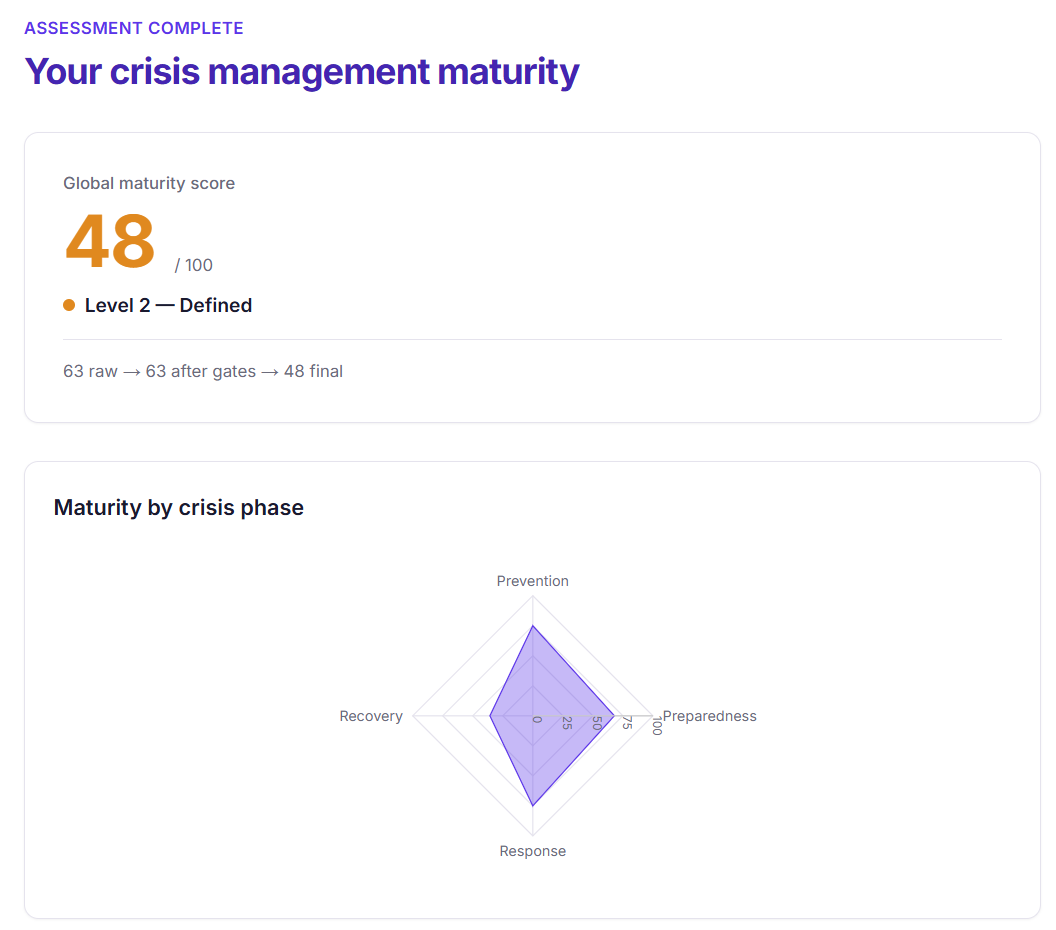
\includegraphics[width=0.72\textwidth]{figures/dashboard-score-radar.png}\\[3mm]
  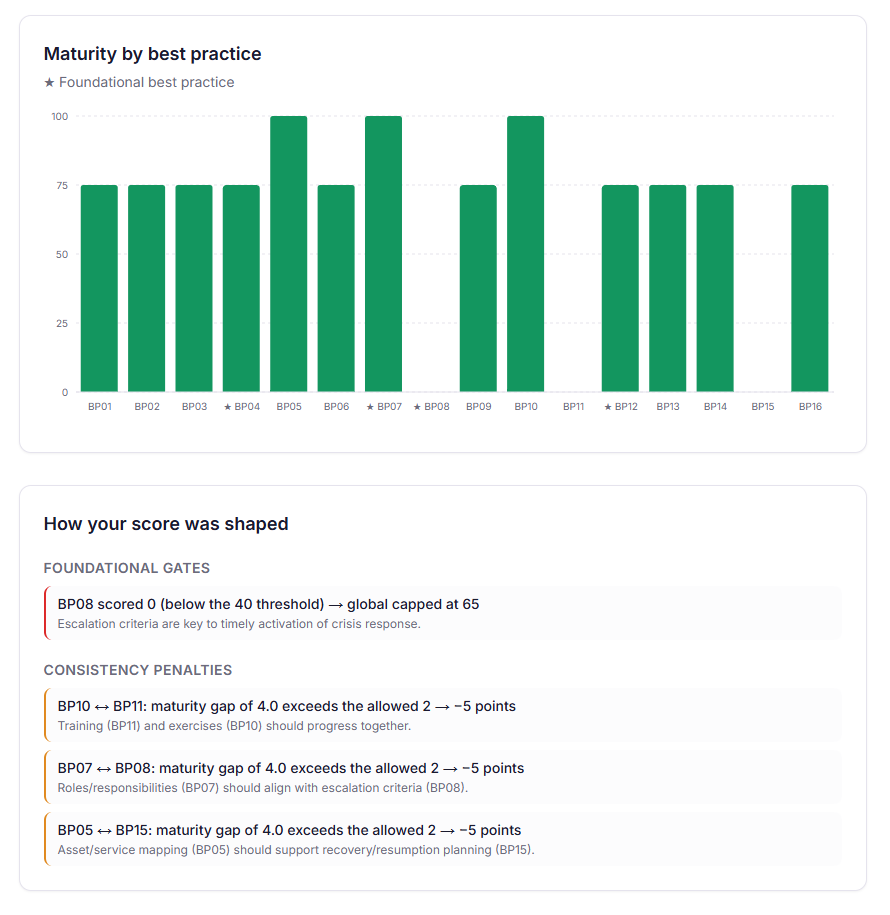
\includegraphics[width=0.72\textwidth]{figures/dashboard-bp-bars.png}
  \caption{Assessment results dashboard: global maturity score and radar chart by phase (top), bar chart by best practice with the foundational gates and consistency penalties that shaped the final score (bottom)}
  \label{fig:frontend-dashboard}
\end{figure}

\subsection{No duplicated framework content, one token layer for theming}

Every component that renders a question or a best-practice name fetches it from \texttt{GET /\allowbreak api/\allowbreak referential} rather than hardcoding it, the same P4 discipline (Chapter~\ref{chap:method}) applied to the frontend: the referential is read once, never copied into a component. Colour follows the same one-place principle, every colour in the interface lives in CSS custom properties in \texttt{app/\allowbreak globals.\allowbreak css}, so re-theming the whole application is a single-file edit. The palette itself is a violet-and-grey scheme inspired by Wavestone's identity, deliberately not copied from the official charter and using no Wavestone logo, which keeps the deliverable presentable to the company without misrepresenting a student project as an official Wavestone product.

\subsection{i18n: English only, no locale routing (for now)}

Text goes through \texttt{next-\allowbreak intl}, but the interface ships in English only, with no URL-prefixed locale routing such as \texttt{/\allowbreak en} or \texttt{/\allowbreak fr}. I considered adding routed locales from the start, since a consulting client base is not necessarily English-speaking, but rejected it as premature for a single-language MVP: every string already goes through a message key, so adding a second language later is a two-line change to a messages file, not a rewrite of any component. The cost of the full routing machinery is deferred until there is a second language to justify it.

None of this is a security boundary. The interface hides screens a user should not see and redirects an unauthenticated visitor to the login page; every protected call still stands on its own behind the checks described in Section~\ref{sec:platform-auth-security}, and a user who reaches an endpoint directly gets exactly the same 401, 403 or 404 the backend would have returned anyway.

% --------------------------------------------------------------
\section{Authentication and security}
\label{sec:platform-auth-security}

Real authentication did not appear all at once. From the first sprint, the backend already carried a full users, organisations and roles schema, and every route already depended on \texttt{Depends(get\_\allowbreak current\_\allowbreak user)}; at that stage the dependency was a stub that read an opaque session cookie and silently created an anonymous \texttt{User} row on first contact (principle P5, Chapter~\ref{chap:method}). The stub existed precisely so that real authentication could later replace one function behind a fixed signature, not force a schema migration or a rewrite of every route. This section covers what replaced it: the invitation cascade that turns an email address into an account, the session model, the roles and the per-owner access control built on top of them, and the concrete security measures that follow from treating a platform handling client organisations' maturity data as something that has to defend itself.

\subsection{Invitation cascade and account activation}

Accounts are never created directly. An admin or a consultant issues a single-use invitation bound to one email address and one role; the recipient turns it into an account by choosing a password at \texttt{POST /\allowbreak api/\allowbreak auth/\allowbreak accept}. I call this option B: an invitation link that leads to a chosen password, as opposed to a passwordless magic link that would log the user in directly. The backend never sends an email itself, \texttt{POST /\allowbreak api/\allowbreak auth/\allowbreak invitations} returns the clear token exactly once and a human relays it out of band, a sequence set out in Figure~\ref{fig:auth-invitation-cascade} in Appendix~\ref{app:figures}. I chose this over building an SMTP integration because the environment genuinely has none configured, and because the consulting workflow is human-driven anyway: a consultant already knows the client they are onboarding and can hand them a link directly. A pure magic link would have avoided a password entirely, but it gives no durable credential for a client who comes back a week later, so option B trades one extra step at signup for a normal login afterwards. The very first admin account is seeded the same way, by \texttt{backend/\allowbreak bootstrap\_\allowbreak admin.\allowbreak py}, which creates an admin invitation with \texttt{invited\_\allowbreak by} left \texttt{NULL}; every other account, including that first admin, is activated through the exact same \texttt{accept\_\allowbreak invitation} path, so there is only one place in the codebase that enforces the password policy and the bcrypt hashing described below.

Who may invite whom is fixed as well: an admin can invite an admin, a consultant or a respondent; a consultant can only invite a respondent; a respondent invites nobody. The role on an activated account comes from the invitation itself, never from the accept request, so a recipient has no way to hand themselves a higher role than the one they were invited with. Invitations are also single-use and time-bounded, a consumed token or an expired one cannot be replayed, which closes off both reusing an old link and leaving a leaked one usable indefinitely.

\subsection{Server-side sessions, not JWT}

Logging in, or accepting an invitation, opens a row in a \texttt{sessions} table and stores only the SHA-256 hash of an opaque random token; the clear token itself rides in an HttpOnly cookie, never reachable from JavaScript. \texttt{get\_\allowbreak current\_\allowbreak user} resolves that cookie to a session and then to a user on every request. The project brief mandated cookie sessions and ruled out JWT, and the case for it holds beyond the brief: a server-side store gives real revocation, logging out, or a future ``kill all sessions'' action, only has to delete the row, so a stolen or copied token dies immediately. A stateless JWT cannot do that without maintaining a blocklist, which is a server-side store by another name, so cookie sessions did not cost anything a JWT would have saved. Every session is also bounded by an \texttt{expires\_\allowbreak at}, regardless of whether it is ever explicitly revoked.

The cookie itself carries three attributes together: HttpOnly (unreachable from JavaScript, closing off token theft through XSS), SameSite=Lax (a first line of defence against CSRF), and Secure, configurable and required in production to stop the cookie riding over plain HTTP. Section~\ref{sec:platform-networking} returns to what SameSite actually cost during development, once the frontend and the backend stopped being the same origin.

\subsection{A problem encountered: passlib versus bcrypt}

The first attempt at password hashing went through \texttt{passlib}, the usual wrapper library, and it broke immediately: \texttt{passlib} 1.7.4 is unmaintained and crashes against \texttt{bcrypt} 5.x, because it inspects a \texttt{\_\allowbreak \_\allowbreak about\_\allowbreak \_\allowbreak .\allowbreak \_\allowbreak \_\allowbreak version\_\allowbreak \_\allowbreak } attribute that no longer exists on the newer package. Rather than pin an old, unmaintained \texttt{bcrypt} version to keep \texttt{passlib} happy, I called \texttt{bcrypt} directly, \texttt{hashpw} and \texttt{checkpw}, and kept that call inside one small, unit-tested module, \texttt{app/\allowbreak core/\allowbreak security.\allowbreak py}. The session and invitation tokens, which are high-entropy random values rather than user-chosen passwords, are hashed with SHA-256 instead: a fast hash is the right tool for an unguessable random value, and \texttt{bcrypt}'s 72-byte input cap together with its per-hash salt would have made a simple equality lookup on a token impossible anyway.

\subsection{Password policy and login hardening}

Three more measures target the login path itself, beyond hashing. A password policy enforces a minimum length, a byte cap (bcrypt silently truncates past 72 bytes, so the policy has to reject what the hash would otherwise ignore), a check against a common-password blocklist, and a minimum character diversity. Every login attempt costs the same amount of work regardless of whether the email exists: an unknown email still runs a dummy bcrypt verification, and \texttt{POST /\allowbreak api/\allowbreak auth/\allowbreak login} returns one generic 401 in every failure case, wrong password, unknown email, or a locked account, so a caller cannot distinguish which one happened. After a fixed number of consecutive failures, the account locks for a fixed number of minutes. Together these close the two classic login-path vulnerabilities: account enumeration through timing or differential responses, and brute-force or credential-spraying against a valid account.

\subsection{Roles and per-owner access control}

By the time real authentication replaced the anonymous stub (Section~\ref{sec:platform-backend}), the role set had narrowed to three: admin, consultant and respondent. Read access is granted to the admin, to the owner of an assessment, or to the owner's consultant; write access is granted only to the admin or the owner, consultants are read-only on their clients' assessments, which matches an advisory role, a consultant guides, the client fills in. Every listing query is scoped in SQL rather than filtered after the fact, and the consultant-to-client link is derived from a single existing relationship, \texttt{Invitation.\allowbreak invited\_\allowbreak by} joined to the activated account by email, instead of a separate organisation or membership table. I preferred deriving the link from data that already existed over adding a new join table: it is the simplest model that expresses ``a consultant sees the clients they onboarded'' for an MVP, and a richer organisation structure can replace it later without changing the shape of the rule itself. The whole rule lives in one module, \texttt{app/\allowbreak core/\allowbreak authz.\allowbreak py}, applied as a FastAPI dependency ahead of every handler, which is a direct answer to OWASP A01, Broken Access Control~\cite{owasp_top10_a01_2021}: the access check that gets forgotten, or that quietly diverges between two endpoints, is overwhelmingly the usual way this category of vulnerability appears, and there is exactly one place to get it right instead of one per route.

One edge case falls out of this rule on its own. Assessments created before authentication existed have no owner, \texttt{user\_\allowbreak id} is \texttt{NULL}, so they match none of the role-scoped read branches and surface only in the admin's unfiltered view. I left it that way rather than guessing an owner to reassign them to: defaulting ownerless data to admin-only is the most restrictive safe choice, and reassigning it by hand later is cheap, whereas a wrong automated guess would have created a silent cross-tenant exposure.

\subsection{401 vs 403 vs 404: denying an existence oracle}

The three denial codes are not interchangeable. A \texttt{401} means the caller is not authenticated at all. A \texttt{403} is used when the caller is authenticated but forbidden from an action on a resource they may legitimately know exists, a consultant attempting to write to a client's assessment, or inviting someone above their own role. A \texttt{404} is used uniformly for both an unknown id and a lack of read access. Returning \texttt{403} on a resource the caller can read but not write is honest, since they already know it exists; returning \texttt{403} on a resource they cannot even read would itself confirm that the id exists, which is exactly the information an outsider probing for valid assessment ids wants. Collapsing ``unknown'' and ``forbidden to read'' into the same \texttt{404} denies that oracle.

\subsection{Defence in depth: the frontend never enforces access}

Section~\ref{sec:platform-frontend} already noted that the interface only adapts to a role, it does not enforce one. The reasoning belongs here: a client-side guard is code a user controls and can simply skip, so it is not a security boundary by definition, and treating it as one would be a false sense of safety. \texttt{lib/\allowbreak auth.\allowbreak ts} mirrors the backend's role hierarchy purely to populate invitation dropdowns with the roles a given user is allowed to grant, and the backend re-checks that choice independently every time; the frontend's actual job is narrower, to avoid rendering a screen that would immediately fail against the checks above. The login and role-gated screens reuse the same design tokens introduced in Section~\ref{sec:platform-frontend} rather than a new colour scheme, which keeps them consistent with the rest of the interface at no extra cost.  Table~\ref{tab:auth-owasp-measures} in Appendix~\ref{app:tables} gathers every measure described in this section alongside the risk it is meant to close, so that the coverage can be read in one pass rather than reconstructed from the prose.

% --------------------------------------------------------------
\section{Local AI integration}
\label{sec:platform-local-ai}

The AI layer sits strictly downstream of the engine. Per the referential's own \texttt{ai\_\allowbreak module\_\allowbreak scope} (\texttt{scoring\_\allowbreak role:\allowbreak  none}), it reads a fully-computed \texttt{Assessment\allowbreak Result} and produces text only: an executive synthesis, a top three-to-five list of prioritised actions, and best-practice-specific recommendations enriched beyond the referential's static fallbacks. It never modifies a score or overrides a deterministic calculation, never infers or imputes a missing answer, and the same scoring input must always yield the same scoring output regardless of what the model does, which is exactly what anti-pattern~3 (Chapter~\ref{chap:method}, letting a non-deterministic component touch a number that has to be defensible) is avoided by construction rather than by discipline. \texttt{app/\allowbreak llm/\allowbreak } talks to Ollama's \texttt{/\allowbreak api/\allowbreak generate} directly over \texttt{httpx}, with no framework in between, consistent with anti-pattern~2 as well.

\subsection{The deployed model and its candidates}

The referential's \texttt{ai\_\allowbreak module\_\allowbreak scope} lists four candidate models, \texttt{mistral:\allowbreak 7b-\allowbreak instruct}, \texttt{mixtral:\allowbreak 8x7b}, \texttt{llama3.\allowbreak 1:\allowbreak 8b} and \texttt{qwen2.\allowbreak 5:\allowbreak 7b}, three of them in the 7 to 8 billion parameter range and the fourth a mixture-of-experts (MoE) model. All four are larger than what the platform actually runs: Ollama runs \texttt{qwen2.\allowbreak 5:\allowbreak 3b} by default, on CPU inside the VirtualBox VM described in Section~\ref{sec:platform-networking}. Table~\ref{tab:ai-model-comparison}, in Appendix~\ref{app:tables}, records each model and what became of it; the arbitration itself came down to latency rather than quality in the abstract, and Chapter~\ref{chap:validation} sets out the figures behind it and the limits of the comparison. The deployed model is one environment variable away from being swapped once a GPU or a larger machine is available.

\subsection{Anti-hallucination guardrails}

Three guardrails keep the model from inventing something a consultant could not defend in front of a client, one upstream of generation and two downstream. Upstream, the prompt anchors the model to the exact best-practice ids the referential defines, and it carries no PII at all, no organisation name, no identifiers, and no N/A justification text, which is principle P3 (Chapter~\ref{chap:method}) applied specifically to what leaves the local boundary. Downstream, the parser canonicalises the \texttt{bp\_\allowbreak id} variants the model might produce, then discards any recommendation that cites a best practice outside the referential; Chapter~\ref{chap:validation} sets out both steps and why a fused id is dropped rather than split.

The scoring engine's independent audit (Chapter~\ref{chap:scoring-engine}) had flagged this exact boundary as worth testing explicitly, ahead of the AI layer being built. The guarantee turned out to be structural rather than a precaution taken only inside the prompt builder: \texttt{na\_\allowbreak justification} exists solely on \texttt{BPAnnotation}, the engine's input side, and the output types the engine actually returns, \texttt{Assessment\allowbreak Result} and \texttt{BPResult} in \texttt{app/\allowbreak scoring/\allowbreak models/\allowbreak outputs.\allowbreak py}, carry no such field, no organisation name and no personal identifier. \texttt{build\_\allowbreak prompt} (\texttt{app/\allowbreak llm/\allowbreak recommendations.\allowbreak py}) only ever receives that computed result together with the referential, never the raw \texttt{Assessment}, \texttt{Organization} or \texttt{User} row, so there is no code path left for a justification to reach the model even by accident. Three tests in \texttt{backend/\allowbreak tests/\allowbreak test\_\allowbreak llm\_\allowbreak privacy.\allowbreak py} lock this down without calling Ollama: one runs a real \texttt{Assessment\allowbreak Input} carrying a sentinel value inside an N/A justification through \texttt{score\_\allowbreak assessment} and then \texttt{build\_\allowbreak prompt}, and asserts the sentinel appears in neither the prompt nor the serialised result; a second asserts structurally that \texttt{Assessment\allowbreak Result} declares no organisation, client name or identifier field at all; a third combines several sentinel types at once to cover more than one category of sensitive data in a single pass. All 71 backend tests pass, including these three, and none of them found a leak. The guarantee depends on the output schema staying narrow, a property the second test locks in place, and should be read as conditional on that schema rather than as an unconditional property of the system.

\subsection{Deterministic fallback}

On any failure from the model, Ollama unreachable, a timeout, or output the parser cannot make sense of, the endpoint degrades to the referential's own static \texttt{fallback\_\allowbreak recommendation\_\allowbreak when\_\allowbreak low\_\allowbreak maturity} text for each weak best practice, and reports \texttt{source="fallback"} so the frontend can be honest about where the text came from (Figure~\ref{fig:ai-pipeline}, Appendix~\ref{app:figures}). The score itself is never at the mercy of this: it is computed and returned by the engine regardless of whether the narrative generation succeeds. The same property is what lets the backend's test suite, and the end-to-end smoke test, run without a live model at all; the fallback path is exercised directly rather than skipped.



\subsection{Asynchronous UX for a slow local model}

Because a single generation takes roughly a minute, the results page cannot simply await it inline. Generated recommendations are cached in memory only, inside a React context living in the root layout, explicitly not \texttt{local\allowbreak Storage} or \texttt{session\allowbreak Storage}. The cache is keyed once per assessment id and reused across navigation within the same browser session, so moving between the dashboard and a detail view does not re-trigger generation, while a full page reload does. I chose in-memory over persisting across reloads for the same reason the score itself is recomputed rather than stored (Section~\ref{sec:platform-backend}): the narrative is reproducible on demand, and persisting it risks showing a stale text once the underlying answers have changed. In-memory caching is the lightest option that removes the one-minute wait from every navigation without introducing a second staleness problem alongside the one the engine already avoids.

% --------------------------------------------------------------
\section{Networking and operational choices}
\label{sec:platform-networking}

The dev and demo setup does not run everything on the same host. The frontend and the backend run inside a VirtualBox NAT virtual machine, while the local model, Ollama, runs on the Windows host that hosts the VM. That single fact, three processes instead of one shared \texttt{localhost}, is the source of every problem in this section: three settings that have to agree, a topology that has to be understood before either of them can be fixed, and one debugging story that took a while to trace back to that topology.

\subsection{The links that must agree}

Three settings have to agree at once for a request to make it from a browser to the engine and back: where the frontend believes the backend is, which origins the backend accepts requests from, and where the backend believes Ollama is. Table~\ref{tab:network-links}, in Appendix~\ref{app:tables}, lists all three, where each is set, and its default. Two further settings matter without being part of the wiring itself: \texttt{OLLAMA\_\allowbreak MODEL} (the model name, \texttt{qwen2.\allowbreak 5:\allowbreak 3b} by default, Section~\ref{sec:platform-local-ai}) and \texttt{OLLAMA\_\allowbreak TIMEOUT\_\allowbreak SECONDS} (300 by default, generous because CPU inference is slow). When all three processes run on one host, the defaults already agree and nothing needs changing; the VirtualBox setup below is the case where they do not.

\subsection{VirtualBox NAT VM topology}


NAT works in both directions here, and the two are worth separating. From the Windows side, the VM is reached through VirtualBox port forwarding, which maps \texttt{localhost:\allowbreak 3000} and \texttt{localhost:\allowbreak 8000} on the host onto the same ports inside the VM, so the browser never needs the VM's own address at all.
Figure~\ref{fig:network-topology} shows the actual topology. From inside a NAT VM, the host machine is reachable at the fixed alias \texttt{10.\allowbreak 0.\allowbreak 2.\allowbreak 2}, so the backend reaches Ollama at \texttt{http:\allowbreak /\allowbreak /\allowbreak 10.\allowbreak 0.\allowbreak 2.\allowbreak 2:\allowbreak 11434} rather than \texttt{127.\allowbreak 0.\allowbreak 0.\allowbreak 1}. That address only works if Ollama is actually listening on every interface on the Windows side, its default binds to loopback only, so \texttt{OLLAMA\_\allowbreak HOST} has to be set to \texttt{0.\allowbreak 0.\allowbreak 0.\allowbreak 0:\allowbreak 11434} and the service restarted, otherwise it only answers the host's own requests and the VM's calls time out. The committed default in \texttt{config.\allowbreak py} stays \texttt{127.\allowbreak 0.\allowbreak 0.\allowbreak 1}, which is what a fully-local run needs, with \texttt{10.\allowbreak 0.\allowbreak 2.\allowbreak 2} documented beside it for the VirtualBox case and set through \texttt{OLLAMA\_\allowbreak BASE\_\allowbreak URL} when the VM is in use; the environment variable is what should change between environments, never the committed file, so switching deployment targets is never a reason to edit code.

\begin{figure}[ht!]
  \centering
  \begin{tikzpicture}[
    box/.style={draw, rounded corners, align=center, minimum width=4.4cm, minimum height=1.1cm, font=\small, fill=white},
    arr/.style={-{Straight Barb[angle=60:2mm]}, thick},
    lbl/.style={font=\scriptsize, align=center, fill=white, inner sep=1pt},
    container/.style={draw, dashed, rounded corners, inner sep=7mm},
    node distance=20mm and 24mm
  ]

  \node[box] (browser) {Browser};
  \node[box, below=of browser] (frontend) {Frontend\\:3000};
  \node[box, below=of frontend] (backend) {Backend API\\:8000};
  \node[box, right=of backend, xshift=18mm] (ollama) {Ollama\\listening on 0.0.0.0:11434};

  \node[container, fit=(frontend)(backend), label={[font=\small]above:VirtualBox NAT VM}] (vmbox) {};
  \node[container, fit=(ollama), label={[font=\small]above:Windows host}] (hostbox) {};

  \draw[arr] (browser) -- (frontend) node[lbl, pos=0.8, right=2mm] {forwarded port\\localhost:3000};
  \draw[arr] (frontend) -- (backend) node[lbl, midway, right=2mm] {\texttt{NEXT\_\allowbreak PUBLIC\_\allowbreak API\_\allowbreak URL}};
  \draw[arr] (backend) -- (ollama) node[lbl, midway, above, sloped] {\texttt{10.\allowbreak 0.\allowbreak 2.\allowbreak 2:\allowbreak 11434} (NAT alias)};

  \end{tikzpicture}
  \caption{Network topology: VirtualBox NAT VM and the Windows host}
  \label{fig:network-topology}
\end{figure}

\subsection{A problem encountered: the SameSite cross-origin cookie, and the same-origin proxy fix}

The symptom appeared only when the browser ran on Windows, reaching the VM through the port-forwarded NAT setup. After creating an account or logging in, \texttt{POST /\allowbreak api/\allowbreak auth/\allowbreak accept} (or \texttt{/\allowbreak login}) returned a clean 200, the account existed on the backend, and the response carried a \texttt{Set-\allowbreak Cookie} header. The very next request, \texttt{GET /\allowbreak api/\allowbreak me}, came back 401. The frontend concluded nobody was logged in and bounced back to \texttt{/\allowbreak login}, so \texttt{/\allowbreak assessments} was never reachable. The cookie was issued, but the browser never sent it back.

The browser's own DevTools carried the full diagnosis. The Network tab, on the \texttt{accept} or \texttt{login} response, showed an explicit warning on the \texttt{Set-\allowbreak Cookie} header: \emph{this attempt to set a cookie via a Set-Cookie header was blocked because it had the SameSite=Lax attribute but came from a cross-site response which was not the response to a top-level navigation}. Decoded, that meant the cookie carried \texttt{Same\allowbreak Site=Lax}, set deliberately for security (Section~\ref{sec:platform-auth-security}), but the browser treated frontend and backend as two distinct sites because they sat on different ports; under \texttt{Same\allowbreak Site=Lax}, a cookie from a cross-site response is only accepted on a top-level navigation, a clicked link that changes the URL, never on a background \texttt{fetch} such as this login call. The cookie was rejected at the point it was set, confirmed by the Application tab showing nothing stored at all. A second, hidden cause made it worse: a line left in \texttt{.\allowbreak env.\allowbreak local} on the VM, \texttt{NEXT\_\allowbreak PUBLIC\_\allowbreak API\_\allowbreak URL=http:\allowbreak /\allowbreak /\allowbreak 127.\allowbreak 0.\allowbreak 0.\allowbreak 1:\allowbreak 8000}, gitignored and specific to that machine, forced the frontend to call the backend by an absolute cross-origin URL, which guaranteed the cross-site behaviour. It also explained why the bug never showed up on my own machine, where that line was simply absent.

The fix removes the cross-origin condition itself rather than weakening the cookie, across three small changes, all on the frontend. A Next.js proxy, added as \texttt{rewrites} in \texttt{frontend/\allowbreak next.\allowbreak config.\allowbreak mjs}, relays every \texttt{/\allowbreak api/\allowbreak :\allowbreak path*} request from the frontend to the backend:

\begin{lstlisting}[caption={Same-origin proxy via Next.js rewrites}, label={lst:nextjs-rewrites}]
async rewrites() {
  return [
    { source: "/api/:path*", destination: `${backend}/api/:path*` },
  ];
}
\end{lstlisting}

with \texttt{backend} read from a \texttt{BACKEND\_\allowbreak ORIGIN} environment variable (default \texttt{http:\allowbreak /\allowbreak /\allowbreak localhost:\allowbreak 8000}), so the target is configurable rather than hardcoded; the relay runs server-side, inside Next.js, and is invisible to the browser. Second, \texttt{frontend/\allowbreak lib/\allowbreak api.\allowbreak ts} now resolves its base URL to an empty string by default, \texttt{process.\allowbreak env.\allowbreak NEXT\_\allowbreak PUBLIC\_\allowbreak API\_\allowbreak URL}, so every call goes out as a relative \texttt{API} path against the frontend's own origin and is picked up by the proxy; the explicit override still exists for a deployment where the frontend would legitimately call a same-site backend directly. Third, the trapped \texttt{.\allowbreak env.\allowbreak local} line on the VM had to be removed, otherwise it would have kept forcing the absolute URL and the first two changes would have made no difference. The cookie itself was never touched: it stays \texttt{Http\allowbreak Only; Same\allowbreak Site=Lax}. I deliberately did not switch to \texttt{Same\allowbreak Site=None}, which would have required HTTPS and weakened the protection, and did not force HTTPS in development either; the cause was the cross-origin call, not the cookie policy, so that is what got fixed.

Figure~\ref{fig:samesite-fix} summarises the change. Once the browser sees a single origin, \texttt{localhost:\allowbreak 3000}, the login exchange is no longer cross-site, \texttt{Same\allowbreak Site=Lax} behaves as intended, the cookie is stored, and \texttt{GET /\allowbreak api/\allowbreak me} carries it back and returns 200; the redirect loop to \texttt{/\allowbreak login} disappeared and the full path, login, list, questionnaire, dashboard, works end to end. As a side effect, this same-origin topology is closer to a production deployment behind a single reverse-proxied domain than the two-port dev setup was, so the fix also removed a difference between dev and production rather than just papering over a local quirk. The files worth citing are \texttt{frontend/\allowbreak next.\allowbreak config.\allowbreak mjs} (the rewrites), \texttt{frontend/\allowbreak lib/\allowbreak api.\allowbreak ts} (the relative base URL), \texttt{frontend/\allowbreak .\allowbreak env.\allowbreak example} (documenting \texttt{BACKEND\_\allowbreak ORIGIN}), and the \texttt{.\allowbreak env.\allowbreak local} trap itself as the reason the bug was VM-specific.  Writing the diagnosis down once, rather than solving it silently and moving on, follows the same instinct as the architecture decisions log referenced throughout this chapter: a problem that cost this much to trace is worth documenting the first time it is solved.

\begin{figure}[ht!]
  \centering
  \begin{tikzpicture}[
    box/.style={draw, rounded corners, align=center, minimum width=3.2cm, minimum height=1.05cm, font=\small},
    arr/.style={-{Straight Barb[angle=60:2mm]}, thick},
    badarr/.style={-{Straight Barb[angle=60:2mm]}, thick, dashed},
    lbl/.style={font=\scriptsize, align=center, fill=white, inner sep=1pt},
    node distance=10mm and 20mm
  ]

  \node[box] (b_browser) {Browser};
  \node[box, right=of b_browser] (b_frontend) {Frontend\\:3000};
  \node[box, right=of b_frontend, xshift=8mm] (b_backend) {Backend\\:8000};

  \draw[arr] (b_browser) -- (b_frontend);
  \draw[badarr] (b_frontend) -- (b_backend)
    node[lbl, midway, above] {absolute URL\\cross-origin};
  \node[lbl, below=1mm of b_backend, text width=3.6cm] {Set-Cookie blocked:\\SameSite=Lax, cross-site};

  \node[font=\small, above=6mm of b_frontend] {Before};

  \node[box, below=28mm of b_browser] (a_browser) {Browser};
  \node[box, right=of a_browser] (a_frontend) {Frontend\\:3000};
  \node[box, right=of a_frontend, xshift=8mm] (a_backend) {Backend\\:8000};

  \draw[arr] (a_browser) -- (a_frontend);
  \draw[arr] (a_frontend) -- (a_backend)
    node[lbl, midway, above] {\texttt{next.\allowbreak config.\allowbreak mjs}\\rewrites, server-side};
  \node[lbl, below=1mm of a_backend, text width=3.6cm] {Cookie accepted:\\single origin, :3000 only};

  \node[font=\small, above=6mm of a_frontend] {After};

  \end{tikzpicture}
  \caption{Before and after the same-origin proxy fix}
  \label{fig:samesite-fix}
\end{figure}

\cleardoublepage{}

\chapter{Validation and Results}
\label{chap:validation}

Chapters 5 and 6 described what the platform is built to do and how it is
built. This chapter asks a different question, whether it actually does what
it claims, and how this was checked. I present the three layers of testing
that support the deterministic engine and the platform built around it, walk
through one concrete assessment profile from raw score to final score,
evaluate the local AI layer against its own guardrails, and close with the
limitations I consider important to state explicitly rather than leave for a
reader to discover on their own.

\section{Validation strategy}
\label{sec:validation-strategy}

The validation approach follows directly from the inviolable principles
introduced in Chapter 4 (\ref{chap:method}), in particular the requirement
that the scoring engine be deterministic and auditable. Testing is organised
in three layers, moving from the pure computation core outward to the full
request path a user actually exercises.

\subsection{Three layers of testing}
\label{subsec:three-layers}

The first layer tests the scoring engine in isolation, as a pure Python
package with no I/O. The second layer tests the FastAPI backend that wraps
it, exercising HTTP endpoints against a real (in-memory) database. The third
layer is a targeted cross-check of the single seam between the two, the
translation from stored, raw answers to the engine's input format.

\begin{table}[htbp]
  \centering
  \begin{tabular}{@{}lll@{}}
    \toprule
    Layer & Scope & Location \\
    \midrule
    Engine unit tests & Pure scoring pipeline, no I/O & \texttt{app/scoring/tests/} \\
    Backend integration tests & FastAPI endpoints, async DB & \texttt{backend/tests/} \\
    End-to-end bridge cross-check & DB row to \texttt{AssessmentInput} to result & \texttt{score\_test.py} \\
    \bottomrule
  \end{tabular}
  \caption{The three testing layers}
  \label{tab:testing-layers}
\end{table}

\begin{figure}[htbp]
  \centering
  \begin{tikzpicture}[
      >=Latex,
      node distance=4mm,
      proc/.style={
        draw=black!65, thick, rounded corners=2pt, fill=black!4,
        minimum height=1.0cm, text width=1.9cm, align=center,
        font=\footnotesize
      },
      data/.style={
        draw=black!55, thick, dashed, rounded corners=2pt, fill=white,
        minimum height=1.0cm, text width=1.9cm, align=center,
        font=\footnotesize\itshape
      },
      band/.style={
        rounded corners=2pt, thick, minimum height=0.85cm
      },
      guide/.style={draw=black!35, dashed, line width=0.5pt},
      lbl/.style={font=\scriptsize, align=center}
    ]

    \node[proc]                          (n1) {HTTP\\request};
    \node[proc, right=of n1]             (n2) {FastAPI\\endpoint + DB};
    \node[proc, right=of n2]             (n3) {scoring\_\\bridge.py};
    \node[data, right=of n3]             (n4) {Assessment\\Input};
    \node[proc, right=of n4]             (n5) {Engine\\(Ch.~5)};
    \node[data, right=of n5]             (n6) {Assessment\\Result};
    \node[proc, right=of n6]             (n7) {HTTP\\response};

    \draw[->] (n1) -- (n2);
    \draw[->] (n2) -- (n3);
    \draw[->] (n3) -- (n4);
    \draw[->] (n4) -- (n5);
    \draw[->] (n5) -- (n6);
    \draw[->] (n6) -- (n7);

    \draw[guide] (n4.south west) -- ++(0,-0.9);
    \draw[guide] (n6.south east) -- ++(0,-0.9);
    \draw[band, draw=blue!55!black, fill=blue!8]
      ($(n4.south west)+(0,-0.9)$) rectangle ($(n6.south east)+(0,-1.75)$);
    \node[lbl, blue!55!black] at ($(n4.south east)!0.5!(n6.south west)+(0,-1.325)$)
      {Engine unit tests};

    \draw[guide] (n2.south west) -- ++(0,-2.0);
    \draw[guide] (n4.south east) -- ++(0,-2.0);
    \draw[band, draw=teal!60!black, fill=teal!8]
      ($(n2.south west)+(0,-2.0)$) rectangle ($(n4.south east)+(0,-2.85)$);
    \node[lbl, teal!60!black] at ($(n2.south east)!0.5!(n4.south west)+(0,-2.425)$)
      {End-to-end bridge\\cross-check};

    \draw[guide] (n1.south west) -- ++(0,-3.1);
    \draw[guide] (n7.south east) -- ++(0,-3.1);
    \draw[band, draw=black!55, fill=black!5]
      ($(n1.south west)+(0,-3.1)$) rectangle ($(n7.south east)+(0,-3.95)$);
    \node[lbl, black!55] at ($(n1.south east)!0.5!(n7.south west)+(0,-3.525)$)
      {Backend integration tests};

  \end{tikzpicture}
  \caption{Overview of the validation pipeline}
  \label{fig:validation-pipeline}
\end{figure}

The engine suite grew from 64 tests at the point of the independent audit
(\ref{chap:scoring-engine}) to 67 after the corrections it triggered, three
new tests specifically targeting a gap the audit had identified (see
\ref{subsec:test-profiles}), and stands at 70 today. The backend suite,
which exercised only the two endpoints required by the end of Sprint 0,
\texttt{test\_health.py} and \texttt{test\_referential\_endpoint.py}, grew
alongside every backend feature landed afterward, assessments, scoring,
authentication and access control, and now counts 68 tests.

\subsection{Deterministic testing philosophy}
\label{subsec:deterministic-philosophy}

Because the engine is deterministic by construction (principle P1, Chapter
4), its tests can assert exact values rather than tolerance ranges. A test
such as \texttt{test\_determinism}, which runs the same assessment through
the engine twice and compares the two serialized outputs, would be
meaningless for a component with any randomness or hidden state. This is
also why the golden scenarios described below assert precise numeric scores
rather than approximate bounds, and why the boundary sweep test can claim
exhaustive coverage of a parameter range rather than sampling it. This
certainty does not extend to the AI layer, which is evaluated on different
terms in \ref{sec:ai-evaluation}.

\subsection{Test profiles built for coverage}
\label{subsec:test-profiles}

Beyond the determinism check, the engine suite is organised around a small
number of named scenarios chosen to exercise specific parts of the scoring
pipeline described in Chapter 5, particularly the parts most likely to hide
a subtle error, ordering, thresholds, and edge conditions.

\begin{table}[htbp]
  \centering
  \begin{tabular}{@{}lp{9cm}@{}}
    \toprule
    Test & Purpose \\
    \midrule
    \texttt{test\_determinism} & Same input run twice yields identical output \\
    Golden scenarios (5) & End-to-end reference cases covering the full pipeline \\
    \texttt{test\_bounds\_across\_sweep} & 20 parametrized combinations, proves the final score stays in $[0, 100]$ \\
    \texttt{test\_evidence\_caps\_are\_strictly\_increasing} & Evidence-type caps are monotonic \\
    \texttt{test\_golden\_na\_is\_neutral} & A N/A best practice contributes to neither numerator nor denominator \\
    Loader validation tests & Missing file, malformed YAML, missing field all raise \\
    \texttt{test\_golden\_consistency\_penalty\_triggered} & A maturity gap above threshold deducts the expected points \\
    \texttt{test\_golden\_two\_gates\_strictest\_cap\_wins} & Two simultaneous foundational gates, the stricter cap is retained \\
    \texttt{test\_penalty\_threshold\_is\_strict\_greater\_than} & A gap exactly at the threshold does not penalize, just above does \\
    \bottomrule
  \end{tabular}
  \caption{Named test scenarios and what each one locks down}
  \label{tab:test-profiles}
\end{table}

The last three rows were added after an independent audit of the engine
found that the consistency-penalty branch, one of the two original
correction mechanisms of the model, was never exercised by any test (finding
H1, \ref{chap:scoring-engine}). This is worth dwelling on briefly. A
64-test suite is a good headline number, but it had a gap precisely where
the model's own differentiating logic lived. The three tests added close
that gap without touching a single line of production code, they capture
the pipeline's existing, correct behaviour rather than changing it.

\section{Functional results}
\label{sec:functional-results}

Where Section~\ref{sec:validation-strategy} described how the platform is
tested, this section shows what those tests actually establish, first about
the seam between storage and computation, then about the scoring pipeline
itself through a single worked example.

\subsection{API-engine cross-check}
\label{subsec:bridge-crosscheck}

The engine suite (Chapter~\ref{chap:scoring-engine}) proves that the scoring
pipeline is correct in isolation, given a well-formed \texttt{AssessmentInput}.
It says nothing about whether the platform actually builds a well-formed
\texttt{AssessmentInput} from what a user submitted. That translation is the
single most likely place for a silent mismatch to appear, a renamed field, a
dropped answer, a best practice marked N/A on one side and not the other, so
it is deliberately isolated in one module, \texttt{scoring\_bridge.py}, rather
than spread across the API layer.

\texttt{scoring\_bridge.py} is the only module in the codebase that imports
both the SQLAlchemy models and the engine's Pydantic input models. Its
\texttt{build\_assessment\_input} function maps a stored \texttt{Assessment}
row, with its answers and best-practice annotations eagerly loaded, into an
\texttt{AssessmentInput}, and \texttt{missing\_answers} independently
precomputes the full list of unanswered questions.

This second function exists because of a risk raised during the engine audit
(Chapter~\ref{chap:scoring-engine}), before the bridge was written, an
incomplete assessment would reach the engine, which raises a bare
\texttt{KeyError} on the first missing answer it encounters rather than
reporting the assessment as incomplete. Left unhandled, this would have
surfaced as an opaque \texttt{500} response. \texttt{missing\_answers} closes
that gap ahead of time, so the scoring endpoint can return every missing
answer at once as a \texttt{422}, keeping genuine user errors out of the
server-error range, as documented in \ref{chap:platform}. This is a small
illustration of a pattern that recurs through the project, a risk identified
on paper is treated as a requirement on the next component, not as an
afterthought once it fails in practice.

\texttt{score\_test.py} exercises this seam end to end, it builds an
assessment through the API, submits answers, requests a score, and checks the
result against what calling the engine directly on the same input would
produce, proving that the bridge introduces no distortion.

\subsection{Worked example: from raw score to final score}
\label{subsec:worked-example}

The scoring pipeline applies, in order, an evidence cap, a phase-weighted
aggregation, a foundational-gate cap, and a consistency-penalty deduction
(Chapter~\ref{chap:scoring-engine}). Each step is unit-tested independently
(Section~\ref{subsec:test-profiles}), but a single assessment profile that
exercises several of them in sequence makes the cumulative effect concrete in
a way that isolated tests do not. This is also, deliberately, the numeric
proof that the engine audit found missing (finding H1,
Chapter~\ref{chap:scoring-engine}), the correction added the test, this
section reports what it actually shows.

Table~\ref{tab:worked-example} follows the \texttt{penalized} test profile
through the pipeline. The four phase scores it produces, 75 for Prevention,
68 for Preparedness, 75 for Response, and 36 for Recovery, average to a raw
global score of 63 under the referential's equal 25 percent phase weighting.
BP08, a foundational best practice, scores 0 on this profile, well below its
40-point threshold, which triggers its foundational gate and caps the global
score at 65. Because the raw score of 63 already sits below that cap, the
gate is recorded as applied but does not move the number, an instructive
edge case, a gate can fire without being the binding constraint. Three
consistency pairs then trigger simultaneously, BP10 against BP11, BP07
against BP08, and BP05 against BP15, each with a maturity gap of 4.0 against
an allowed maximum of 2, each deducting 5 points. The three penalties bring
the score down by 15 points in total, from 63 to a final global score of 48
(48.4 before rounding), mapped to maturity level 2, Defined.

\begin{table}[htbp]
  \centering
  \begin{tabular}{@{}lr@{}}
    \toprule
    Stage & Score \\
    \midrule
    Raw global score & 63 \\
    After foundational gate & 63 \\
    After consistency penalties & 48 \\
    Final global score & 48 \\
    \bottomrule
  \end{tabular}
  \caption{Worked example: the \texttt{penalized} profile}
  \label{tab:worked-example}
\end{table}

This example is a useful counterpoint to a purely additive reading of the
model. A respondent looking only at individual best-practice scores could
reasonably expect a global score closer to the mid-sixties. The gap between
that expectation and the actual 48 is exactly the point of the two
correction mechanisms, a single very weak foundational best practice and a
pattern of inconsistent maturity across related practices both leave a
visible mark on the final number, which is the intended, auditable
behaviour rather than a computational surprise.

\section{AI evaluation}
\label{sec:ai-evaluation}

The scoring engine can be validated the way Sections~\ref{sec:validation-strategy}
and~\ref{sec:functional-results} did it, against exact expected values, because
it is deterministic. The local AI layer is not, and evaluating it calls for
different terms, the reasoning behind the model choice, the guardrails put in
place because the model cannot be trusted unsupervised, how often those
guardrails have to intervene, and a qualitative read of what the output is
actually worth.

\subsection{Model selection: qwen2.5:3b versus a 7B model}
\label{subsec:model-selection}

Ollama is configured to run \texttt{qwen2.5:3b} by default rather than a
larger model such as \texttt{mistral:7b-instruct}, one of the candidates
originally listed for this role (\texttt{referential.yaml},
\texttt{ai\_module\_scope}). The reasoning is documented in the architecture
log, inference runs on CPU inside the demo VM, where a 7B model's latency
made the recommendations endpoint impractical, multi-minute responses
observed informally rather than through a controlled benchmark, while
\texttt{qwen2.5:3b} keeps generation to approximately one minute. This is
defensible because the task given to the model is constrained rather than
open-ended, it summarizes and enriches recommendations that the referential
already supplies for a handful of weak best practices, it does not reason
freely over the whole framework.

Even at roughly a minute, blocking the dashboard on generation was not
acceptable, which is why recommendations are fetched asynchronously and
cached in memory per assessment, the dashboard renders immediately and the
narrative fills in once ready, fetched once and reused across navigation
rather than regenerated on every visit (\ref{chap:platform}). The model
choice and this caching decision address the same constraint from two
directions, one lowers the cost of a generation, the other lowers how often a
generation has to happen at all.

The trade-off is left open rather than closed, the model is swapped through a
single environment variable, and a controlled, timed comparison against a
larger model remains future work (\ref{subsec:perspectives-future-work}).

\subsection{Failure modes and guardrails}
\label{subsec:failure-modes}

A 3B model prompted to reference specific best-practice identifiers is not a
reliable source of exact strings, so the AI layer is built on the assumption
that it will occasionally get an identifier wrong rather than on the hope
that it will not. The scoring role is fixed regardless, the model receives a
fully computed \texttt{AssessmentResult} and produces text only, it never
touches a score (principle P1, \ref{chap:scoring-engine}). The prompt is
anchored to the exact list of best-practice identifiers relevant to the
assessment and carries no personally identifiable information, no
organization name, no identifiers, no N/A justification text (principle P3).

Two guardrails sit downstream of generation, before any text reaches the
user. First, identifier normalization corrects the shapes a small model
tends to produce, a bare \texttt{BP4} is padded to \texttt{BP04}, but a fused
identifier such as \texttt{BP123} is rejected outright rather than guessed
apart into \texttt{BP01} and \texttt{BP23}, since splitting it would be
fabricating a claim the model never actually made about either practice.
Second, every normalized identifier is checked for existence against the
loaded referential, an action citing a best practice that is not in the
framework, such as a fabricated \texttt{BP18} on a referential that only
defines sixteen, is discarded rather than shown.

The result is that a hallucinated identifier or a malformed response is a
degraded response, not an incorrect one, the worst case is losing the
AI-generated narrative for that best practice, never seeing a fabricated one.
This existence check is scoped to the full referential rather than to the
narrower subset of weak best practices sent in a given prompt, a distinction
worth naming explicitly in Section~\ref{subsec:ai-quality-limitation}.

\subsection{Residual fallback rate}
\label{subsec:fallback-rate}

The guardrails in Section~\ref{subsec:failure-modes} are only as reassuring
as they are infrequently needed, a system that falls back on every request
would be technically safe but practically equivalent to not having an AI
layer at all. This frequency was not tracked systematically during
development, no instrumentation logged how often the endpoint actually
returned \texttt{source="fallback"} across real or test invocations, so no
rate can be reported here. The fallback path was directly observed at least
once during testing, for the assessment discussed in
Section~\ref{subsec:worked-example}, which returned the referential's
static recommendations rather than an AI-generated narrative
(Section~\ref{subsec:qualitative-ai}). One observed instance says nothing
about frequency, but it does confirm the fallback path is exercised in
practice and not merely a theoretical branch. This absence of a tracked rate
is itself worth naming rather than papering over, and it points to concrete
follow-up work, instrumenting the recommendations endpoint to log its own
degradation rate would turn this qualitative observation into a measurable
one. Once a network misconfiguration between the demo VM and the host
running Ollama was diagnosed and corrected, a successful AI-generated
response was also obtained on the same profile, confirming that both the
fallback path and the AI path are exercised in practice rather than one
being purely theoretical (Section~\ref{subsec:qualitative-ai}).

\subsection{Qualitative assessment of recommendations}
\label{subsec:qualitative-ai}

The referential's static text is a fixed sentence per best practice,
independent of how the organization actually answered
(\texttt{fallback\_recommendation\_when\_low\_maturity},
\texttt{referential.yaml}). The AI layer's stated responsibility is to go
beyond that, to produce an executive synthesis in natural language, to
prioritize the three to five actions that matter most across the weak best
practices found, taking foundational status and dependencies into account,
and to contextualize each recommendation using what the user actually
answered rather than the generic text alone
(\texttt{ai\_module\_scope.downstream\_responsibilities},
\texttt{referential.yaml}).

Table~\ref{tab:recommendation-comparison} compares both outputs on the same
\texttt{penalized} profile discussed throughout this chapter, static referential
text against the AI-generated narrative for the same three priority best
practices, BP08, BP11, and BP15.

\begin{table}[htbp]
  \centering
  \small
  \begin{tabular}{@{}p{1.8cm}p{7cm}p{7cm}@{}}
    \toprule
    Field & Static (referential fallback) & AI-generated (\texttt{qwen2.5:3b}) \\
    \midrule
    Executive summary &
    Overall crisis-management maturity is assessed at 48.4/100, level 2,
    Defined. Focus first on the priority actions below, which target the
    weakest and most structural best practices. &
    The organization's cyber crisis management is below par, with scores
    averaging at level 2, Defined. Key priorities include establishing
    clear escalation criteria for timely activation of plans, implementing
    a comprehensive training program for cyber crisis managers, and
    developing robust Business Resumption Plans. \\
    \addlinespace
    BP08 &
    Define operational escalation criteria, severity, scope, time
    pressure, translate into decisions, who, when, how, and test in
    exercises. Foundational best practice, score 0.0/100. &
    Define operational escalation criteria including severity, scope, and
    time pressure, and test in exercises. Timely activation is crucial to
    effective response, establishing clear guidelines will improve
    readiness. \\
    \addlinespace
    BP11 &
    Implement a training curriculum for cyber crisis roles, including
    onboarding, regular sessions, and effectiveness measurement. Score
    0.0/100. &
    Implement a training curriculum for cyber crisis roles with regular
    sessions and effectiveness measurement. Continuous training ensures
    staff are prepared, aligning responsibilities with escalation
    criteria. \\
    \addlinespace
    BP15 &
    Develop an integrated BRP with BCP/DR, regular review, recovery tests,
    and stakeholder involvement beyond IT. Score 0.0/100. &
    Develop an integrated Business Resumption Plan aligned with the
    Business Continuity Plan and Disaster Recovery Plan, including regular
    reviews and stakeholder involvement beyond IT. Resilience planning is
    critical for recovery, a comprehensive BRP ensures a coordinated
    approach to business continuity. \\
    \bottomrule
  \end{tabular}
  \caption{Static referential text against AI-generated narrative, same
  profile, same three best practices}
  \label{tab:recommendation-comparison}
\end{table}

The comparison is more modest than the stated ambition. For all three
actions, the AI output is close to a paraphrase of the static text rather
than a substantively new recommendation, BP08 keeps the same three criteria
in the same order, BP11 keeps the same structure with one clause dropped,
BP15 mostly expands the acronyms. What the AI genuinely adds is a short
justification sentence appended to each action, absent from the static
version, explaining in general terms why the action matters. This is a real
addition, but a generic one, the justification for BP08 or BP11 would read
just as naturally attached to a different weak best practice, it is not
visibly grounded in this organization's specific pattern of failure, three
triggered consistency penalties on top of one marginal foundational gate
(\ref{subsec:worked-example}).

The executive summary shows a comparable trade, the AI version drops the
precise 48.4 score present in the static text in favour of a looser
paraphrase, "scores averaging at level 2", which is imprecise in a way the
static text is not, the final score is not a simple average, it results from
the gate and penalty mechanism described in
Section~\ref{subsec:worked-example}. No identifier was fabricated and no
best practice outside the referential's sixteen was cited in this instance,
so the guardrails held, but holding the guardrails and adding genuine
analytical value are two different bars, and on this single example the
output clears the first more convincingly than the second.

\section{Limitations}
\label{sec:limitations}

The guardrails and cross-checks described in the previous sections make the
platform trustworthy within a defined scope. They do not make the underlying
model of maturity itself complete. Four limitations are worth stating plainly
rather than leaving for a reader to find, because each one bears directly on
how much weight a result from this tool should be given.

\subsection{Self-assessment is inherently declarative}
\label{subsec:declarative-limitation}

Every score the platform produces ultimately rests on what a respondent
chooses to answer. Nothing in the data model requires, or is able to require,
that a declared maturity level of 3 for a given question actually reflects
the organization's practice rather than the respondent's understanding of it,
or their incentive to present it favourably. This is not a flaw specific to
this implementation, it is a property of self-assessment as a method, shared
with essentially every maturity framework that does not involve an external
auditor collecting evidence directly. The platform inherits it rather than
solves it, and the two mitigations built against it, evidence caps and the
consistency penalties, are best understood as bounding the damage a purely
declarative answer can do to the score, not as removing the underlying
dependency on honest, informed self-reporting.

\subsection{The evidence cap mitigates declarativeness only partially}
\label{subsec:evidence-cap-limitation}

The evidence-type mechanism (\ref{chap:scoring-engine}) caps a declared
maturity level according to the strongest evidence category the respondent
selects, an unsupported claim cannot score above level 1, a claim backed by a
real incident can reach level 4. This meaningfully narrows how far a purely
declarative answer can inflate a score. It does not close the gap entirely,
because the evidence type itself is self-selected in exactly the same way
the maturity level is, the data model records which category the respondent
chose, not any independent proof that the category is accurate. A respondent
willing to overstate a maturity level is equally free to overstate the
evidence behind it, and the platform has no upload, audit trail, or
verification step that would catch this. The cap changes the shape of the
incentive to inflate a score, it does not remove it.

\subsection{No inter-rater reliability study}
\label{subsec:interrater-limitation}

The scoring engine's determinism guarantees that the same answers always
produce the same score (\ref{chap:scoring-engine}). It says nothing about
whether two different, equally informed people answering on behalf of the
same organization would give the same answers in the first place. No study
was run to check this, no assessment was completed independently by more
than one respondent from the same organization and compared. Without that
data, a claim that the tool measures maturity objectively, rather than
measuring one respondent's perception of it consistently, would be
overstated. This is a natural extension for validating the methodology
further, not a defect in what was built during the internship.

\subsection{AI output quality not formally measured beyond anchoring constraints}
\label{subsec:ai-quality-limitation}

Section~\ref{sec:ai-evaluation} established that the AI layer cannot corrupt
a score and cannot cite a best practice outside the referential, both
verified properties. That second guarantee is narrower than it first
appears, it checks membership in the sixteen-best-practice referential as a
whole, not membership in the smaller set of weak best practices actually
sent to the model for a given assessment (\ref{subsec:failure-modes}). A
real but contextually irrelevant identifier would currently pass this check
undetected, a gap that stops short of a hallucinated global score or a
fabricated best practice, but is narrower than the guarantee as informally
described.

Neither guarantee says anything about whether the generated narrative is
actually good advice, whether the prioritization across weak best practices
is sound, whether the contextualization beyond the static fallback text is
genuinely more useful to a reader than the fallback would have been on its
own. The single worked comparison in Section~\ref{subsec:qualitative-ai}
suggests the current output leans closer to paraphrase than to genuine
contextualization, but one example is an illustration, not a formal
evaluation. Evaluating that properly would require either a domain expert
scoring a larger sample of generated recommendations against some rubric, or
feedback from someone who used the tool in a real advisory context, neither
of which was carried out. What Section~\ref{sec:ai-evaluation} demonstrates
is that the AI layer is safe to expose, not that its output has been shown
to be good, and the two claims should not be conflated.

Taken together, these four limitations describe the boundary of what this
internship validated, and what it did not have the time or the setting to
validate. None of them undermine the platform's core claim, that a
deterministic, auditable score can be computed from structured self-reported
answers, but they do bound how that score should be interpreted and by whom.
Chapter~\ref{chap:pm} returns to several of these points from a project
management angle, in particular what a next iteration would prioritize given
more time.

\cleardoublepage{}

\chapter{Impact, Value, and Perspectives}
\label{chap:impact}

Chapter~\ref{chap:validation} showed what the platform does and does not establish: the scoring engine computes what it specifies, within a suite of tests and an independent audit, and the AI layer was shown to be safe to expose, with its output checked against the referential before it reaches a user, while the usefulness of that output was never formally evaluated. This chapter steps back from that validation to ask a different question, what the resulting tool is actually worth, to Wavestone, to the client organisations it targets, and to the broader question of how LLMs can be used responsibly in a sensitive domain, before closing on the directions left open for a project delivered within the bounds of a single internship.

\section{Value for the consulting practice}
\label{sec:impact-consulting}

Within the bounds Chapter~\ref{chap:validation} sets out, this section turns to what the platform is worth to the practice that commissioned it. The value described here follows three related lines: a more defensible starting point for client conversations, the time and consistency gained from a repeatable instrument, and a shared vocabulary between consultant and client.

\subsection{A defensible starting point for client conversations}
\label{sec:impact-consulting-starting-point}

The difficulty set out in Section~\ref{sec:gap} is what the platform addresses directly: a self-assessment grounded in the ENISA best practices, discussed at length in Chapter~\ref{chap:state-of-the-art} and Chapter~\ref{chap:context}, produces a first, structured read of where an organisation stands before a consultant even walks into the room. Informal feedback gathered from two practitioners in Wavestone Luxembourg's Cyber practice, an analyst and a manager both regularly involved in running crisis management exercises, supports this reading. Their recurring difficulty, in their own account, is establishing where a given organisation actually stands before designing an exercise or a mission around it, and both saw the tool as directly useful for that purpose, in particular for identifying the best practices where an organisation is weakest, information that can then be used to design an exercise that genuinely tests those gaps rather than one that confirms strengths already in place.

\subsection{Time savings and consistency across engagements}
\label{sec:impact-consulting-time-savings}

Two related benefits follow from the deterministic nature of the scoring engine (Chapter~\ref{chap:scoring-engine}, principle P1 in Chapter~\ref{chap:method}). First, a consultant no longer needs to build an assessment structure from scratch for each engagement: the referential and the scoring pipeline already exist and only need to be run against a given organisation's answers. Second, because the same inputs always produce the same score regardless of who runs the assessment, the tool removes a source of inconsistency that is otherwise hard to avoid when maturity is judged qualitatively by different consultants on different engagements. Neither benefit has been measured quantitatively at this stage, and no claim is made here about a specific amount of time saved.

\subsection{A shared methodological language}
\label{sec:impact-consulting-shared-language}

By turning the sixteen ENISA best practices into named, identifiable units, BP01 to BP16, organised into four phases and scored on a common zero-to-four maturity scale, the platform gives consultants and clients, the intended audience described in Chapter~\ref{chap:framing}, a shared vocabulary to talk about crisis management maturity. A finding expressed as ``BP08 is at maturity level 1'' is unambiguous and reproducible in a way that a purely narrative assessment is not, which in turn makes it easier for a consultant and a client's security or governance team to agree on what needs to improve and why.

The observations above draw on informal, internal feedback rather than on a supervised client trial: at the time of writing, the platform has not been used on an actual client engagement, and no decision, formal or informal, has been made regarding whether or how Wavestone might use it going forward. The value described here is therefore best read as an informed expectation grounded in early internal reactions from practitioners, not as a demonstrated commercial outcome.

\section{Value for client organisations}
\label{sec:impact-clients}

Section~\ref{sec:impact-consulting} looked at value from Wavestone's side of the table. The same platform, run against a client's own answers, offers three related benefits to the organisation being assessed: a self-assessment explicitly aligned with the framework NIS2 implicitly expects, a set of recommended actions anchored in that same framework rather than in generic advice, and a score whose derivation the client, or an external auditor, can inspect rather than simply trust.

\subsection{A NIS2-aligned self-assessment}
\label{sec:impact-clients-nis2-alignment}

For an organisation subject to NIS2, the practical difficulty is less the existence of the directive's crisis management expectations than the absence of an instrument to translate them into a concrete, measurable position. The referential underlying this platform operationalises exactly the framework NIS2 implicitly relies on for crisis management capability, the ENISA ``Best Practices for Cyber Crisis Management'' study discussed in Chapter~\ref{chap:context} and Chapter~\ref{chap:state-of-the-art}. Running a self-assessment against this referential gives a client organisation a structured, repeatable way to locate itself relative to that framework ahead of, rather than during, external scrutiny. The alignment operates at the level of the framework as a whole: the referential already carries per-best-practice fields intended for article-level NIS2 mapping (Section~\ref{sec:impact-perspectives}), but these remain unpopulated at the time of writing, so no claim is made here about article-by-article legal compliance.

\subsection{Prioritised, framework-anchored actions}
\label{sec:impact-clients-prioritised-actions}

A raw maturity score is of limited use on its own; what a client organisation needs is a sense of where to act first. The scoring pipeline already surfaces this through its foundational gates (Chapter~\ref{chap:scoring-engine}), which cap the overall score when a foundational best practice is under-developed, and the AI recommendation layer built strictly downstream of the score (Chapter~\ref{chap:platform}, principle P1 in Chapter~\ref{chap:method}) turns the weakest best practices into narrative guidance. The result a client receives is therefore a short, prioritised list of actions anchored in the same referential used to compute the score, rather than a generic checklist assembled independently of the assessment.

\subsection{An auditable, defensible score}
\label{sec:impact-clients-auditable-score}

Because the score is produced by a deterministic engine kept strictly separate from the AI layer (Chapter~\ref{chap:method}), it can be reconstructed from the underlying answers at any time, and the reasoning behind it, the audit trace described in Chapter~\ref{chap:scoring-engine}, is available for inspection rather than hidden inside a model's output. Determinism is locked down by a dedicated test that scores the same input twice and compares the results byte for byte, and the engine as a whole went through an independent audit before any platform work began (Chapter~\ref{chap:scoring-engine}). For a client organisation, this matters concretely: a score a security team can defend to its own management, or to an external auditor, is worth more than one it can only assert.

\section{Technological impact}
\label{sec:impact-technological}

Beyond its value to Wavestone and to client organisations, the project also makes a narrower technological point, less specific to crisis management and more about how LLMs can be used responsibly in a sensitive, regulated context. Two observations follow from the choices described in Chapter~\ref{chap:method} and revisited in Chapter~\ref{chap:validation}.

\subsection{A local LLM producing structured, on-topic output in a sensitive context}
\label{sec:impact-technological-local-llm}

The literature reviewed in Chapter~\ref{chap:state-of-the-art} frames model selection as a trade-off between fidelity, latency and infrastructure cost, smaller models running on commodity hardware against larger ones requiring dedicated GPU resources. This project puts that trade-off under a concrete constraint rather than treating it only in principle: a small, CPU-run, fully local model, deployed through Ollama (Chapter~\ref{chap:platform}) and never exposed to client data or PII (principle P3, Chapter~\ref{chap:method}), produced recommendations structured and on-topic enough to be usable for this specific task, on the qualitative reading reported in Chapter~\ref{chap:validation}, a single worked comparison made by the author on one assessment profile rather than a formal evaluation with external reviewers or an agreed rubric. This is not a general claim that small local models suffice for any LLM-augmented task; the task here is narrow and well-scoped, turning an already-computed set of weak best practices into narrative guidance, rather than open-ended reasoning. Within that scope, however, it is a concrete demonstration that structured, on-topic output does not require sending sensitive assessment data to a cloud provider, which matters directly for organisations operating under NIS2's data-handling expectations.

\subsection{Deterministic computation, AI strictly downstream: a reusable pattern}
\label{sec:impact-technological-pattern}

The second observation concerns architecture rather than model choice. The strict separation between a deterministic scoring engine, treated as the sole source of truth, and an LLM confined to producing narrative text on top of an already-computed result (principles P1 and P3, Chapter~\ref{chap:method}) was motivated by the hallucination risk documented in Chapter~\ref{chap:state-of-the-art}. Nothing in this separation is specific to crisis management maturity: the same pattern, compute a defensible result first with conventional logic, then let an LLM explain or prioritise that result rather than produce it, could plausibly extend to other domains where an organisation needs an auditable output alongside natural-language assistance, such as other maturity or compliance assessments. This project instantiates that pattern once, in one domain; it does not itself constitute evidence that the pattern has been, or will be, reused elsewhere at Wavestone.

\section{Perspectives and future work}
\label{sec:impact-perspectives}

This final section shifts from what was built to what could follow. One item below is not really a perspective at all: authentication was built during the internship and is already part of the platform, and is included here only to mark that boundary before turning to what remains open. Everything else in this section is a direction identified by the author as worth pursuing, not a commitment from Wavestone or a scheduled piece of work; none of it has an agreed timeline at the time of writing.

\subsection{Already in place: authentication and access control}
\label{sec:impact-perspectives-authentication}

Real authentication, invitation-based account creation, server-side cookie sessions, three roles and per-owner assessment isolation, was itself once an open item and is now fully built, described in Chapter~\ref{chap:platform}. It is listed here, out of order with the rest of this section, only to draw a clear line: everything that follows is envisaged, not delivered.

\subsection{NIS2 and ISO/IEC 27035 mapping}
\label{sec:impact-perspectives-nis2-iso-mapping}

The referential reserves, for every best practice, a \texttt{nis2\_articles} and an \texttt{iso\_27035\_clauses} field intended to record which article of the directive and which clause of the standard that best practice operationalises (Chapter~\ref{chap:scoring-engine}, first introduced in Chapter~\ref{chap:state-of-the-art}). At the time of writing these are empty placeholders, ready to receive such a mapping but carrying none for any of the sixteen best practices. As noted in Section~\ref{sec:impact-clients-nis2-alignment}, the platform's NIS2 alignment currently operates at the level of the ENISA framework as a whole; populating these fields would move it toward article- and clause-level granularity, and would most usefully be done with input from someone with regulatory or standards expertise rather than as a purely technical exercise.

\subsection{Retrieval-augmented generation over the ENISA/NIS2 corpus}
\label{sec:impact-perspectives-rag}

The current AI layer grounds its recommendations in the assessment's own structured output through prompt grounding, discussed in Chapter~\ref{chap:state-of-the-art}, rather than in retrieval over source documents. A RAG approach, indexing the ENISA and NIS2 texts with a vector store and Ollama embeddings and letting the model draw on that corpus when producing recommendations, was identified early in the project as a possible direction and left open at the time of writing. Beyond the engineering effort, it would raise the same question already flagged for the previous item: recommendations that cite specific passages of a regulatory or normative text carry a higher expectation of accuracy, and would need validation against the mitigation strategies discussed in Chapter~\ref{chap:state-of-the-art} rather than being assumed to reduce hallucination by construction.

\subsection{Tracking maturity over time and cross-client benchmarking}
\label{sec:impact-perspectives-versioning-benchmarking}

Each assessment result is currently computed on demand from a set of answers and never stored as a standalone record (Chapter~\ref{chap:method}). This is adequate for a single assessment but leaves two related ideas unaddressed. The first is tracking a given client's maturity over time, for instance re-running the same assessment annually and showing how each best practice has evolved, which would require storing successive results rather than only the answers behind them. The second is benchmarking across clients, positioning one organisation's maturity against others in the same sector once enough assessments exist, which would require aggregating and anonymising results from several clients, a data-governance question of its own that has not been designed and that would need to respect the same privacy discipline already applied to the AI layer (principle P3, Chapter~\ref{chap:method}).

\subsection{Infrastructure hardening and end-to-end testing}
\label{sec:impact-perspectives-hardening-testing}

Two infrastructure items remain open. A Docker Compose setup was planned from the project's first sprint but never built; the backend already resolves its referential path through an overridable environment variable for exactly this purpose, but no compose file packages the three services together. A migration from SQLite to PostgreSQL is planned for the same post-MVP stage flagged in Chapter~\ref{chap:platform}; since the backend already uses an async SQLAlchemy stack, this would in principle only require changing the \texttt{DATABASE\_URL} the application points at, though this has not been attempted. Separately, the existing test suites cover the scoring engine and the backend API in isolation (Chapter~\ref{chap:scoring-engine}, Chapter~\ref{chap:platform}); no end-to-end test exercises the full assessment flow through the actual frontend, a gap that closing would give more confidence in the platform as a whole rather than in its parts individually.

\cleardoublepage{}

\chapter{Project Management and Critical Reflection}
\label{chap:pm}
\emergencystretch=3em\relax

The preceding chapters have presented the platform itself, its scoring engine, its architecture, and the results obtained from it. This chapter turns from what was built to how it was built, and to what I would keep or change about that process. The internship brief asks explicitly for a description of the working method and project management approach followed, and for a critical look back at my own work, and I take both requirements seriously here. Section~\ref{sec:pm-working-method} revisits the method described in Chapter~\ref{chap:method} in light of what actually happened, Section~\ref{sec:pm-risks} recounts the main difficulties encountered and how each was resolved, Section~\ref{sec:pm-differently} is a frank account of what I would do differently with the benefit of hindsight, and Section~\ref{sec:pm-skills} closes on the skills the project mobilised and the ones it left me with. I have tried throughout to resist the temptation to smooth the account into a success story, an engineering project is judged as much by how its difficulties were handled as by its final state.

\section{Working method, in retrospect}
\label{sec:pm-working-method}

Chapter~\ref{chap:method} described the method chosen at the outset of the project, sprint-bounded increments, five inviolable principles, and a documentation-first discipline meant to keep the reasoning behind each choice legible. This section does not repeat that description, it asks how well the method actually held once the work was underway, and where it needed to bend.

\subsection{Sprint-bounded work and the Definition of Done}
\label{sec:pm-sprints}

Development proceeded through short, explicitly scoped sprints, tracked as tagged milestones in the project's git history (\texttt{sprint-0}, \texttt{sprint-0b-scoring-api}, and later the smaller \texttt{AUTH.1} to \texttt{AUTH.3} mini-sprints for authentication). Each sprint carried its own definition of done, a short list of what had to work end to end before moving on, rather than a general intention to make progress on several fronts at once. In practice this discipline held up well for the highest-risk piece of the project: integrating the pre-existing scoring engine into a real backend and database, rather than the frontend or the deployment stack, was treated as the priority to de-risk first, and the sprint boundaries made that priority explicit and enforceable rather than aspirational.

The tags say what was done in which order, they do not say when, and a working method is hard to judge without the calendar it ran against. The internship ran for six months, from 9 March to 8 September 2026, and Table~\ref{tab:pm-timeline} sets out the project's main phases in the sequence in which they were actually carried out, from the design of the scoring engine through to the writing of this report. One feature of that sequence is worth pointing out before the table itself: the engine was specified, built and independently audited before any platform work started, which is why its audit sits ahead of the first backend sprint rather than appearing later as a review of something already integrated.

\begin{table}[htbp]
  \centering
  \begin{tabular}{@{}>{\raggedright\arraybackslash}p{0.26\textwidth}>{\raggedright\arraybackslash}p{0.17\textwidth}p{0.48\textwidth}@{}}
    \toprule
    Phase & Period & State at close \\
    \midrule
    Referential and scoring engine & Mar.--Apr. 2026 & \texttt{referential.\allowbreak yaml} and the deterministic engine specified and implemented from the ENISA framework, with their own test suite. \\
    Independent audit and corrective loop & Apr. 2026 & Five findings raised and corrected, referential bumped from version 1.0.0 to 1.1.0, engine suite grown from 64 to 67 tests. \\
    Backend construction (\texttt{sprint-0}) & May 2026 & Data model carrying users, organisations and roles, referential loading, API skeleton. \\
    Assessment storage and scoring API (\texttt{sprint-0b}) & May 2026 & Assessment storage with autosave, and the scoring endpoint wired end to end through the engine. \\
    Frontend and end-to-end integration & May 2026 & Next.js client built on top of the completed backend and connected to it: questionnaire, autosave, and the results dashboard. \\
    Authentication and access control (\texttt{AUTH.1}--\texttt{AUTH.3}) & June 2026 & Invitation-based account creation, server-side cookie sessions, three roles, per-owner isolation of assessments. \\
    Local AI recommendation layer & June 2026 & Recommendations generated by a local model through Ollama, strictly downstream of the computed score, with identifier guardrails and a deterministic fallback. \\
    Writing of this report & July--Aug. 2026 & This document, drawn from the dated decision log described in Section~\ref{sec:pm-documentation-first}. \\
    \bottomrule
  \end{tabular}
  \caption{The project's main phases, in the order they were carried out}
  \label{tab:pm-timeline}
\end{table}

\subsection{Documentation-first as a working discipline}
\label{sec:pm-documentation-first}

Alongside the code, two documents were maintained throughout the project and read at the start of every working session: \texttt{CLAUDE.md}, a single reference describing the project's context, principles, and current state, and \texttt{ARCHITECTURE.md}, a running, dated log of methodological and architectural decisions, each entry recording not only what was decided but why. Writing this log at the time a decision was made, rather than reconstructing it months later for the report, is the discipline I would credit most directly for making this chapter, and several others, possible to write with any precision. The cost was real: every non-trivial decision meant pausing to write a paragraph explaining it, which slowed the pace of purely technical progress in the moment. The benefit only became visible in retrospect, when drafting the report required no memory reconstruction, only a search through an existing log.

\subsection{Verification before commit}
\label{sec:pm-verification}

The project also carried a consistent discipline of verifying a decision or a piece of code before treating it as final. Before any of that, the engine had been subjected to an audit carried out independently of its implementation, described in Chapter~\ref{chap:scoring-engine}. Its own test suite was then kept green throughout its move into the backend, and an end-to-end script, \texttt{score\_test.py}, cross-checks the full database-to-engine path against the engine called directly, to catch any distortion introduced by the translation layer between the two. What belongs here is the discipline it reflects: treating a component as trustworthy only once it had been checked by something other than the reasoning that produced it in the first place.

\subsection{Where the method drifted from the plan}
\label{sec:pm-plan-drift}

The method did not, however, hold to its own plan without adjustment, and that departure is worth recording honestly rather than glossing over. Sprint 0's original brief explicitly scoped the scoring endpoint and answer submission out of its definition of done, deferring them to a later sprint, while placing the frontend, the Docker Compose stack, and the accompanying Makefile inside it. What actually happened reversed that order: two sub-sprints, 0B.1 and 0B.2, delivered assessment storage with autosave and the scoring endpoint wired end to end through the engine first, while the frontend, the container stack, and the Makefile were not yet built. I chose to keep the git history's actual order in this report rather than the order originally planned, which forces an admission that the initial plan was not a good predictor of where the real risk lay. In hindsight the reprioritisation was the right call, the scoring engine's integration was the single largest technical risk in the project and it made sense to prove it worked before investing in a user interface for it, but the honest lesson is that the plan itself should have said so from the start, rather than being corrected after the fact.

\subsection{Supervision and stakeholder feedback}
\label{sec:pm-supervision}

The account so far is written in the first person, which risks making the project sound more solitary than it was. The work was carried out under two forms of supervision running on different rhythms, and a few of the decisions reported in this document were settled outside my own judgement.

On the industrial side, I held a point with my supervisor at Wavestone Luxembourg, introduced in Chapter~\ref{chap:framing}, every two weeks. Those meetings were built around a demonstration rather than a written status report: showing the current state of the platform actually running, followed by a short review of what had been done since the previous point and what came next. Working to a fortnightly demonstration had an effect on the work itself that is worth naming, since it meant each increment had to reach a state that could be shown end to end, which is a stricter bar than a component being finished in isolation, and it kept the definition of done described in Section~\ref{sec:pm-sprints} honest rather than nominal.

On the academic side, I reported to my supervisor at TELECOM Nancy by email once a month, and presented the work in person at a mid-internship meeting held before July. That meeting had two outcomes: a review of what had been built at that point, and the validation of the outline of this report, which fixed the structure the document still follows.

Not every decision recorded here was mine to make, and the clearest case is the authentication model discussed in Chapter~\ref{chap:platform}. The project brief mandated cookie-based sessions and ruled out JSON Web Tokens, so that choice was settled before I reached it. What was left to me was to examine whether the constraint held up on its own terms, which is why that section argues the case for server-side sessions on the merits instead of simply recording an instruction, and the argument is stronger for having been tested against an alternative I was not free to take. Feedback also reached the project from outside the supervision line: the two practitioners whose reactions are reported in Chapter~\ref{chap:impact} gave the only reading of the tool from people who would plausibly use it, and it is reported there rather than here because it bears on what the tool is worth rather than on how the project was run.


\section{Risks and difficulties encountered}
\label{sec:pm-risks}

Two risks were identified before the work started, and both were answered by a decision taken up front rather than by a reaction later. The first was the integration of the scoring engine into a real backend and database. The engine was written as a pure, standalone component, and nothing guaranteed that its translation into a persisted, API-driven application would preserve its behaviour; it was the piece the project could least afford to get wrong, and the response was to schedule it first, ahead of the interface and the deployment stack, as Section~\ref{sec:pm-sprints} describes. The second was the reproducibility of the score. An assessment returning a different figure for the same answers would have failed the requirement the whole project rests on, so determinism was fixed as a principle before any code existed (Chapter~\ref{chap:method}), the AI layer was confined strictly downstream of the computation, and the engine was submitted to an independent audit before being integrated anywhere (Chapter~\ref{chap:scoring-engine}).

Both anticipations held. It is worth being equally clear that the difficulties recorded below were not among them: the corporate environment, the reliability of a small local model, and the dependency and configuration incidents that follow were all met in the course of the work rather than foreseen at its start, as was the mismatch between the plan's scope and the time available discussed in Section~\ref{sec:pm-plan-drift}. That asymmetry is worth noting in its own right. The risks I could name in advance were the ones internal to the component I was building, where prior work gave me something to reason from, while those that cost the most time came from the environment around it, where it did not.

This section consolidates the difficulties that cost the most time or exposed a real gap in the working method, most of them already documented as they were resolved. The technical mechanics of each are detailed in the chapters where the corresponding component is described, what I keep here is the retrospective, what each difficulty actually cost, and what it taught me about the way I was working.

\subsection{Corporate environment constraints}
\label{sec:pm-corporate-constraints}

Two constraints tied to working on a corporate machine, distinct from the VM's network wiring described in Chapter~\ref{chap:platform}, shaped the development environment before a single line of the platform was written.

The first, introduced in Chapter~\ref{chap:framing}, was the absence of administrator rights on the Wavestone laptop, which left no usable development environment directly on the host. The only way to get a machine I could freely install and configure software on was to run one myself, inside a virtual machine. The VirtualBox VM was therefore not a choice made for comfort or isolation, it was the only environment left once native development was ruled out, and it is also, by extension, the reason the whole NAT networking setup described in Chapter~\ref{chap:platform} (Ollama reachable from the VM at \texttt{10.0.2.2}) existed at all.

The second was narrower but just as concrete: on the corporate network, \texttt{pip install} simply did not go through. I do not know exactly what was filtering it, and I would rather leave that unstated than guess at a mechanism I never verified, but the effect was unambiguous, package installation failed on the Wavestone connection and succeeded once I tethered through my phone instead. Working around it meant treating a personal mobile connection as part of the development toolchain, a small but telling illustration of what a locked-down corporate network actually costs day to day.

Neither constraint was severe enough to threaten the project, but both forced detours that would not have existed on a personal machine, and both ended up shaping decisions, the VM itself and the networking setup built on top of it, that I would not otherwise have had to make.

\subsection{The SameSite/proxy cookie bug}
\label{sec:pm-cookie-bug}

The most disruptive bug of the project surfaced only on the corporate VM setup, not on my personal machine. After logging in or creating an account, the authentication request itself succeeded, the backend issued a session cookie, but the very next call to \texttt{GET /api/me} came back \texttt{401}, which sent the interface straight back to the login screen in an unbreakable loop. Chapter~\ref{chap:platform} details the mechanics of the fix, what matters here is what the episode cost and what it taught me.

The cause combined a deliberate security setting with an accidental one, both set out in Chapter~\ref{chap:platform}: a cookie policy chosen on purpose, and an unversioned, VM-specific entry in a local \texttt{.env.local} file that pushed every API call onto an absolute cross-origin URL. That second half is precisely why the bug only ever appeared on the VM and never on my own machine, and the fix removed the cross-origin condition rather than weakening the cookie.

Two lessons stayed with me from this. First, a flow this central deserves to be exercised in the actual target configuration early, not just on a comfortable development machine, the bug was invisible until I tested inside the VM setup that the demo would actually run on, and by then it cost real time to trace back to its cause. Second, local configuration files that are deliberately left out of version control, exactly because they are supposed to be machine-specific, are also exactly the kind of thing that produces a bug nobody else can reproduce and that the log rarely explains on its own. I now treat any environment variable that changes behaviour silently as something to double-check explicitly before assuming a bug is somewhere else.

\subsection{Hardware arbitration for the local model}
\label{sec:pm-model-arbitration}

The choice of \texttt{qwen2.5:3b} as the deployed model, discussed from the design side in Chapter~\ref{chap:method} and revisited in Chapter~\ref{chap:validation}, was in practice an arbitration made under a hard constraint rather than a broad comparison. The demo ran on CPU inside a VM, with no GPU available, and \texttt{qwen2.5:7b}, the 7B version of the same model, pushed generation time into several minutes per request, which made the recommendations endpoint impractical to use or to demonstrate. The 3B model kept generation to roughly a minute, still slow but usable.

The honest limitation is that this was a latency-driven decision made against a single comparison, not a benchmark. Of the four candidates listed at the start of the project, \texttt{mistral:7b-instruct}, \texttt{mixtral:8x7b}, \texttt{llama3.1:8b} and \texttt{qwen2.5:7b}, only \texttt{qwen2.5:7b} was ever installed and timed on the project's hardware; the other three were never run at all. Comparing two sizes of one family is the cleanest shape a single comparison can take, since only the parameter count varies, but it remains a single comparison. I stand by the choice given the constraint, a model nobody can wait for is not a useful demo regardless of how much better its output might be, but I would not present it as a rigorously benchmarked trade-off, and Chapter~\ref{chap:validation} is explicit about the same limitation.

\subsection{Reliability of a small local model}
\label{sec:pm-model-reliability}

A 3B-parameter model is a small model, and treating its output as reliable enough to show a user required accepting that it would sometimes be wrong, then designing around that rather than assuming it away. The task it was given is narrow by design, summarising and enriching a short list of already-computed, weak best practices rather than reasoning openly over the assessment, which is precisely what makes a small model viable here at all. Even so, the three guardrails described in Chapter~\ref{chap:platform}, anchoring generation to the listed best-practice identifiers upstream, then normalising and checking every identifier the model returns downstream, together with the fallback to the referential's static recommendations on any failure, exist because I could not treat the model's output as trustworthy by default. The lesson I take from this is less about the specific model and more about the posture: a local, small, non-deterministic component can still be shipped responsibly, but only if the surrounding system is built to assume it will occasionally misbehave, not as an afterthought bolted on once it did.

\subsection{A broken dependency: \texttt{passlib} versus \texttt{bcrypt}}
\label{sec:pm-passlib}

A smaller but telling incident: the plan was to hash passwords through \texttt{passlib}, a well-known abstraction over several hashing backends, which turned out to be unmaintained and to crash outright against a current \texttt{bcrypt} release, for the reason Chapter~\ref{chap:platform} sets out. The fix was to call \texttt{bcrypt} directly instead, which turned out to be fewer moving parts for the same guarantee. The incident cost little time to fix once diagnosed, but it is a small, concrete example of a risk that a completely unlocked dependency set carries throughout a project, taken up more generally in Section~\ref{sec:pm-differently}.

\subsection{Re-authenticating the test tooling}
\label{sec:pm-test-script}

The internal script used to generate test assessments, \texttt{generate\_\allowbreak test\_\allowbreak assessments.py}, populating profiles such as \texttt{perfect}, \texttt{zero}, \texttt{realistic}, \texttt{gated}, \texttt{penalized}, or \texttt{with\_na} for testing and for the dashboard screenshots in Chapter~\ref{chap:platform}, was written before authentication existed, at a time when creating an assessment through the API required no session at all. Once the AUTH.2 sprint locked the assessment endpoints down, requiring a valid session and stamping the caller as owner, the script started failing with \texttt{401 Unauthorized} on every attempt to create an assessment.

The fix was straightforward once diagnosed: the script now takes credentials as arguments, logs in against \texttt{/api/auth/login} first, and reuses the resulting session cookie for the calls that follow. What is worth keeping from the episode is what the failure meant, more than the fix itself. It was not a bug, it was the access control working exactly as designed, refusing an unauthenticated caller regardless of whether that caller was a real user or my own tooling. Security applied consistently does not carve out an exception for the tools built to test it, and finding that out through my own script breaking is, if anything, a better confirmation that the access-control layer described in Chapter~\ref{chap:platform} was doing its job than any test written to prove it deliberately would have been.

\section{What I would do differently}
\label{sec:pm-differently}

This section looks further back, at what I would change if I were starting the project again. Several of the choices revisited here were reasonable given what was known at the time, and I say so explicitly rather than judging them purely with hindsight. The chapter's brief asks for lucidity here, and I have tried to hold to that without turning ordinary trade-offs into failures.

\subsection{A locked Python environment from the start}
\label{sec:pm-lockfile}

The dependency management decision made at the start of the project, plain \texttt{pip} and \texttt{setuptools} against a \texttt{pyproject.toml}, with no lockfile, was reasoned at the time: for an MVP with a short dependency list and a single developer, it was the path with the least extra tooling, to be revisited once the team or the dependency graph grew. With hindsight I would separate two things that are easy to conflate here.

The \texttt{passlib} incident described in Section~\ref{sec:pm-passlib} would not have been avoided by a lockfile. The incompatibility sits at the root, and that wall appears whenever the two libraries are paired, locked or not. A lockfile could only have postponed the discovery by pinning an older, compatible \texttt{bcrypt}, which trades one problem for another rather than solving anything. The actual lesson from that incident is about which dependencies to pick, not about how strictly their versions are pinned.

What a lockfile would genuinely have bought me is reproducibility across the two machines I actually worked on, the Wavestone VM on Python 3.11 and a personal computer whose Python version drifted from it over time, in a setting where installing packages at all was already constrained by the corporate network described in Section~\ref{sec:pm-corporate-constraints}. Pinning exact versions once would have removed an entire class of ``works on one machine, not the other'' bugs that a short dependency list does not make disappear on its own, it only makes them rarer.

\subsection{Benchmarking model sizes earlier}
\label{sec:pm-benchmark-earlier}

Section~\ref{sec:pm-model-arbitration} already owns up to how narrow that comparison was. If I were to redo this part of the project, I would put a small, even rough, benchmark across families as well as sizes on the actual target hardware early, before committing to one, rather than stopping at the first pair that settled the question. It would not have changed the outcome, a CPU-only VM was never going to run a 7B model comfortably, but it would have turned one timing into a documented comparison, which matters for a report whose whole premise is that choices should be traceable and justified rather than merely reasonable in hindsight.

\subsection{Investing in documentation earlier}
\label{sec:pm-documentation-earlier}

Section~\ref{sec:pm-documentation-first} credits the documentation-first discipline, dated decisions logged in \texttt{ARCHITECTURE.md} alongside a living \texttt{CLAUDE.md}, with making this report possible to write with any precision. What is worth adding honestly is that this discipline was not there from the first commit. A working framework existed early, a sprint brief and a set of working rules in \texttt{CLAUDE.md}, but the practice of logging each decision, dated, with its reasoning, only became systematic once backend construction started; the scoring engine itself, together with its independent audit, predates it entirely.

That timing is the one I would change. The scoring engine is the densest part of the project in terms of methodological decisions, the fixed order of the pipeline, the foundational gates, the consistency penalties, the corrections that came out of the audit, and it is exactly the part where I later had to reconstruct some of that reasoning after the fact rather than simply consulting a log, which is both slower and less reliable than writing it down when the decision was still fresh. If anything, this makes the case for documentation-first stronger, not weaker: I am not arguing for it in the abstract, I experienced its absence firsthand at the start of the project.

\section{Skills mobilised and acquired}
\label{sec:pm-skills}

This project drew on skills built up over the engineering curriculum at TELECOM Nancy and through prior projects, and it also required learning several things I did not know how to do before starting. Both sides are worth naming explicitly. Neither list claims to be exhaustive, and distinguishing what I brought to the project from what it taught me is itself part of the critical account this chapter asks for.

\subsection{Skills mobilised from prior training}
\label{sec:pm-skills-mobilised}

Four areas of prior training carried directly into this project, identified at its outset in the subject and skills analysis drawn up at the start of the internship and confirmed by how the work actually unfolded.

Programming skills built through the TELECOM Nancy curriculum, Python in particular, and a general familiarity with JavaScript-based web frameworks, carried directly into both halves of the platform, the Python scoring engine and backend, and the Next.js frontend described in Chapter~\ref{chap:platform}. Prior exposure to security, risk analysis and an understanding of common threat classes, underpinned the access-control and authentication work covered in the same chapter, in particular the OWASP-driven reasoning behind the 401/403/404 policy and the centralised authorisation module. Familiarity with Linux environments, built up before the internship, was exercised constantly, given that the whole platform was developed and run inside a Linux VM for the reasons discussed in Section~\ref{sec:pm-corporate-constraints}; prior exposure to containerisation with Docker was mobilised more partially, since, as Chapter~\ref{chap:impact} notes, the project's own Docker Compose stack remains a planned rather than a built piece of the platform. Finally, the ability to work independently and to communicate progress and constraints to different stakeholders, a general project management skill rather than a technical one, was exercised throughout, from navigating the corporate environment constraints in Section~\ref{sec:pm-corporate-constraints} to gathering the informal practitioner feedback discussed in Chapter~\ref{chap:impact}.

\subsection{Skills newly acquired}
\label{sec:pm-skills-acquired}

Several areas were genuinely new, and most of them map onto specific decisions documented earlier in this report. Deterministic scoring, designing and implementing a scoring pipeline whose output is fully reproducible and auditable from raw inputs, precisely because it is not allowed to depend on anything probabilistic, is the clearest example, and it is the subject of Chapter~\ref{chap:scoring-engine} in its entirety. Integrating a local large language model as a constrained advisory component, rather than as an open-ended assistant, required learning prompt design and output filtering specifically aimed at keeping a non-deterministic component safe to expose, anchoring generation to a fixed set of identifiers and discarding anything outside them, as described in Chapter~\ref{chap:platform} and reflected on in Section~\ref{sec:pm-model-reliability}. Methodological audit is another: having the scoring engine reviewed independently of its own implementation, and acting on the findings rather than treating the review as a formality, described in Chapter~\ref{chap:scoring-engine}, was not something I had practised before this project. Applied security architecture, translating a secure-by-design intent into concrete mechanisms, server-side sessions, centralised access control, password hashing, rather than leaving it as a stated principle, is covered across Chapter~\ref{chap:platform}. Finally, the project required building a working knowledge of the ENISA and NIS2 regulatory and methodological landscape, covered in Chapter~\ref{chap:context} and Chapter~\ref{chap:state-of-the-art}, specific enough to translate into a scoring framework rather than staying at the level of general awareness.

\cleardoublepage{}

\chapter{Conclusion}

\cleardoublepage{}
\renewcommand{\tocbibname}{Bibliographie / Webographie}
\bibliography{bibliography}
\bibliographystyle{plain}

\cleardoublepage{}

\listoffigures
\cleardoublepage{}

\listoftables
\cleardoublepage{}

\lstlistoflistings{}
\cleardoublepage{}

\printnoidxglossaries{}

\cleardoublepage{}
\renewcommand{\thesubsection}{\Roman{subsection}}

\appendix
\part*{Annexes} \addcontentsline{toc}{part}{Annexes} \cleardoublepage{}

\chapter{Première Annexe}
\cleardoublepage{}

\chapter{Seconde Annexe}

\cleardoublepage{}
\thispagestyle{empty}

\section*{Résumé}
\addcontentsline{toc}{chapter}{Résumé}

La directive NIS2 impose aux entités essentielles et importantes de démontrer
leur capacité de gestion de crise cyber plutôt que de l'affirmer. L'étude
\emph{Best Practices for Cyber Crisis Management}, référence européenne publiée
par l'ENISA en février 2024, structure la discipline en seize bonnes pratiques
sur quatre phases, mais reste descriptive, sans échelle, sans standard de
preuve, sans moyen d'en mesurer l'application. Les instruments de maturité
existants, conçus indépendamment, ne se calquent pas sur sa structure. Mené au
sein de la practice Cyber de Wavestone Luxembourg, ce travail transforme le
cadre ENISA en plateforme d'auto-évaluation opérationnelle. Le cadre tient dans
un fichier de spécification unique : quarante-huit questions couvrant les seize
bonnes pratiques, quatre phases pondérées à parts égales, une échelle de
maturité 0--4, des plafonds bornant le niveau déclaré par la preuve invoquée,
des verrous sur quatre bonnes pratiques fondamentales et des pénalités
d'incohérence entre pratiques liées. Un moteur déterministe en Python pur
calcule le score depuis ce seul fichier et les réponses, selon un ordre de
traitement fixe. Il a fait l'objet d'un audit méthodologique dont les
recommandations ont été intégrées, portant la spécification en 1.1.0. Une
plateforme web l'entoure : couche de traduction unique entre stockage et calcul,
authentification sur invitation, sessions côté serveur, trois rôles,
cloisonnement par propriétaire. Un modèle de langage exécuté localement chez
l'utilisateur reste strictement en aval du résultat calculé, ne reçoit aucune
donnée identifiante, voit sa sortie vérifiée contre la spécification et se
replie sur des recommandations statiques en cas d'échec. L'ensemble est couvert
par 141 tests automatisés, dont 70 pour le moteur et 71 pour l'API et
l'intégration. Le score est reproductible et auditable, dans des limites
énoncées : l'auto-évaluation reste déclarative, ses seuils relèvent du jugement
d'expert plutôt que d'une calibration, et la qualité du texte généré n'a pas été
mesurée.

  {\bf Mots-clés~:} gestion de crise cyber, auto-évaluation de maturité,
  scoring déterministe, modèle de langage local

\section*{Abstract}
\addcontentsline{toc}{chapter}{Abstract}

The NIS2 directive expects essential and important entities to demonstrate a
cyber crisis management capability rather than simply assert one. ENISA's
\emph{Best Practices for Cyber Crisis Management}, the European reference of
February 2024, organises the discipline into sixteen best practices across four
phases, yet remains descriptive, specifying what good practice looks like
without providing a scale, an evidence standard, or any way to measure
adherence. Existing maturity instruments were designed independently of it and
do not map onto its structure. This work, carried out within Wavestone
Luxembourg's Cyber practice, turns the ENISA framework into an operational
self-assessment platform. The framework is encoded in a single specification
file: forty-eight questions across the sixteen best practices, four phases
weighted equally, a maturity scale from zero to four, caps bounding a declared
level by the evidence claimed, gates on four foundational best practices, and
penalties for inconsistent maturity between related practices. A deterministic
engine, in pure Python, computes the score from that file and the respondent's
answers alone, following a fixed pipeline order. It went through a
methodological audit whose recommendations were integrated, taking the
specification from version 1.0.0 to 1.1.0. A web platform surrounds the engine,
with a single translation seam between storage and computation,
invitation-based authentication, server-side sessions, three roles and
per-owner isolation. A language model running locally on the user's hardware is
confined strictly downstream of the computed result, receives no identifying
data, has its output checked against the specification, and degrades to static
recommendations on failure. The whole is covered by 141 automated tests,
seventy for the engine and seventy-one for the API and integration. The
resulting score is reproducible and auditable within stated limits: the
assessment remains declarative, its thresholds rest on expert judgement rather
than calibration, and the quality of the generated narrative was not formally
evaluated.

  {\bf Keywords~:} cyber crisis management, maturity self-assessment,
  deterministic scoring, local large language model

\printSignatures

\end{document}
